\chapter{Selection and Categorisation}
\label{chap:selection_and_categorisation}
\chapterquote{Science never solves a problem without creating ten more.}
{George Bernard Shaw, 1856 -- 1950}

\section{Description}

A description of the selection and categorisation under two schemes � a robust cut-based driven approach (used later for the spin) and a highly optimized, standard model specific multivariate method (used later for the nominal analysis and the sideband background method). This would also include the validation procedure with Z->ee decays.

\textbf{15 pages}

\textbf{Brief outline of the three analyses being discussed and their uses}

This thesis presents results of three different analyses used in the Higgs to two photon search at CMS. The nominal results and properties are obtained from the so called \MFM analysis which uses multivariate methods optimised specifically to search for a \SM Higgs boson to select and categorise events. Two further analyses are presented as cross checks to the baseline \MFM analysis. The first, the \CiC analysis, is designed for simplicity and robustness as a cut based approach and, owing to its low level of model dependence, is used for the spin analysis. The second, the \SMVA analysis, serves to cross check the background, the most significant unknown in a search like this, and categorisation by extracting the background under the signal region from sidebands in the diphoton invariant mass spectrum.

Both the \CiC and \MFM analyses have a fully parametric definition of the diphoton invariant mass spectrum where the signal shape is derived from \MC. The \SMVA uses a cut and count method. 


% ---- SECTION ----
\section{Event selection}
\label{sec:event_selection}

There are two complimentary event selections used in the three analyses. The \CiC analysis uses a cut based photon selection whilst the \MFM and \SMVA analyses uses a series of \BDTs to first select photons and then select events. The ultimate aim is a selection which accepts two prompt photons (i.~e.~ does not contain any fakes) and exploits regions of phase space which have a narrow mass resolution and high signal to background ratio.

\subsection{Selection using cuts in categories}
\label{sec:cic}

Cuts are optimised for photons in four non-overlapping categories to take advantage of the different photon energy resolution between the barrel and the endcap and between converted and non-converted photons. The categories are defined as $|\eta|<1.444$ or $|\eta|>1.556$ and $R_{9}<0.94$ or $R_{9}\geq 0.94$ and the cuts are chosen in the following way,

\begin{itemize}
  \item A set of loose cuts are defined as the starting values
  \item The ``N-1" distribution of each cut variable are produced. This is the distribution of each variable after the cuts on all other variables have been applied.
  \item A smooth curve is fitted to the distribution of $S/B$ ratio versus the cut variable
  \item The cut value is chosen by evaluating the curve for the required value of $S/B$
  \item Do the same for all the other variables
\end{itemize}

Consequently a stable set of cut values is obtained by iterating this procedure a few times. Each cut will remove event with the same purity ($S/B$) and thus the efficiency for selected photons is maximise for the chosen purity level. As a result the cuts in the endcap are much tighter than in the barrel, similarly the cuts for low \rnine photons are much tighter than the cuts for high \rnine photons. The cut variables are described below and the cut values shown in Table~\ref{tab:cic_cuts}. The cut setting procedure is optimised on a signal sample of \Hgg MC (with \mH=120\GeV) and a background sample of \gjet events. The photon efficiency of the cuts for the four different classes of photon are shown in Figure~\ref{fig:cic_efficiency} as a function of the supercluster position, \eta, and the photon \pT.

\begin{itemize}
  \item \textbf{PF isolation sum, chosen vertex} - Sum of particle flow photon, charged and neutral hadron isolation sums defined in Sec.~\ref{sec:iso} where all \PF candidates originate from the primary vertex selected in Sec.~\ref{sec:vtx_reco}
  \item \textbf{PF isolation sum, worst vertex} - As above but where all \PF candidates originate instead from the vertex which gives the largest charged hadron PF isolation sum. This add protection for cases when the primary vertex is incorrectly assigned.
  \item \textbf{Charged PF isolation sum} - Described above in Sec.~\ref{sec:iso}
  \item \boldmath{$\sigma_{i\eta i\eta}$} - Described above in Sec.~\ref{sec:photon_presel}
  \item \boldmath{$H/E$} - Described above in Sec.~\ref{sec:photon_presel}
  \item \boldmath{$R_{9}$} - Described above in Sec.~\ref{sec:ecal}
\end{itemize}

\begin{table}[htbp]
  \begin{center}
    \begin{tabular}{|l|c|c|c|c|}
      & \multicolumn{2}{c}{barrel} & \multicolumn{2}{|c|}{endcap} \\ 
      \hline
      & \multicolumn{1}{l|}{\rnine $>$ 0.94} & \multicolumn{1}{l|}{\rnine $<$ 0.94 } & \multicolumn{1}{l}{\rnine $>$ 0.94 } & \multicolumn{1}{|l|}{\rnine $<$ 0.94 } \\ 
      \hline
      PF isolation sum, chosen vertex & 6 & 4.7 & 5.6 & 3.6 \\ 
      \hline
      PF isolation sum, worst vertex & 10 & 6.5 & 5.6 & 4.4 \\ 
      \hline
      Charged PF isolation sum & 3.8 & 2.5 & 3.1 & 2.2 \\ 
      \hline
      $\sigma_{i\eta i\eta}$ & 0.0108 & 0.0102 & 0.028 & 0.028 \\ 
      \hline
      H/E & 0.124 & 0.092 & 0.142 & 0.063 \\ 
      \hline
      \rnine & 0.94 & 0.298 & 0.94 & 0.24 \\ 
    \end{tabular}
  \end{center}
  \caption{Photon ID selection cut values. The cuts are applied to both the leading and subleading photons.}
  \label{tab:cic_cuts}
\end{table}

\begin{figure}
  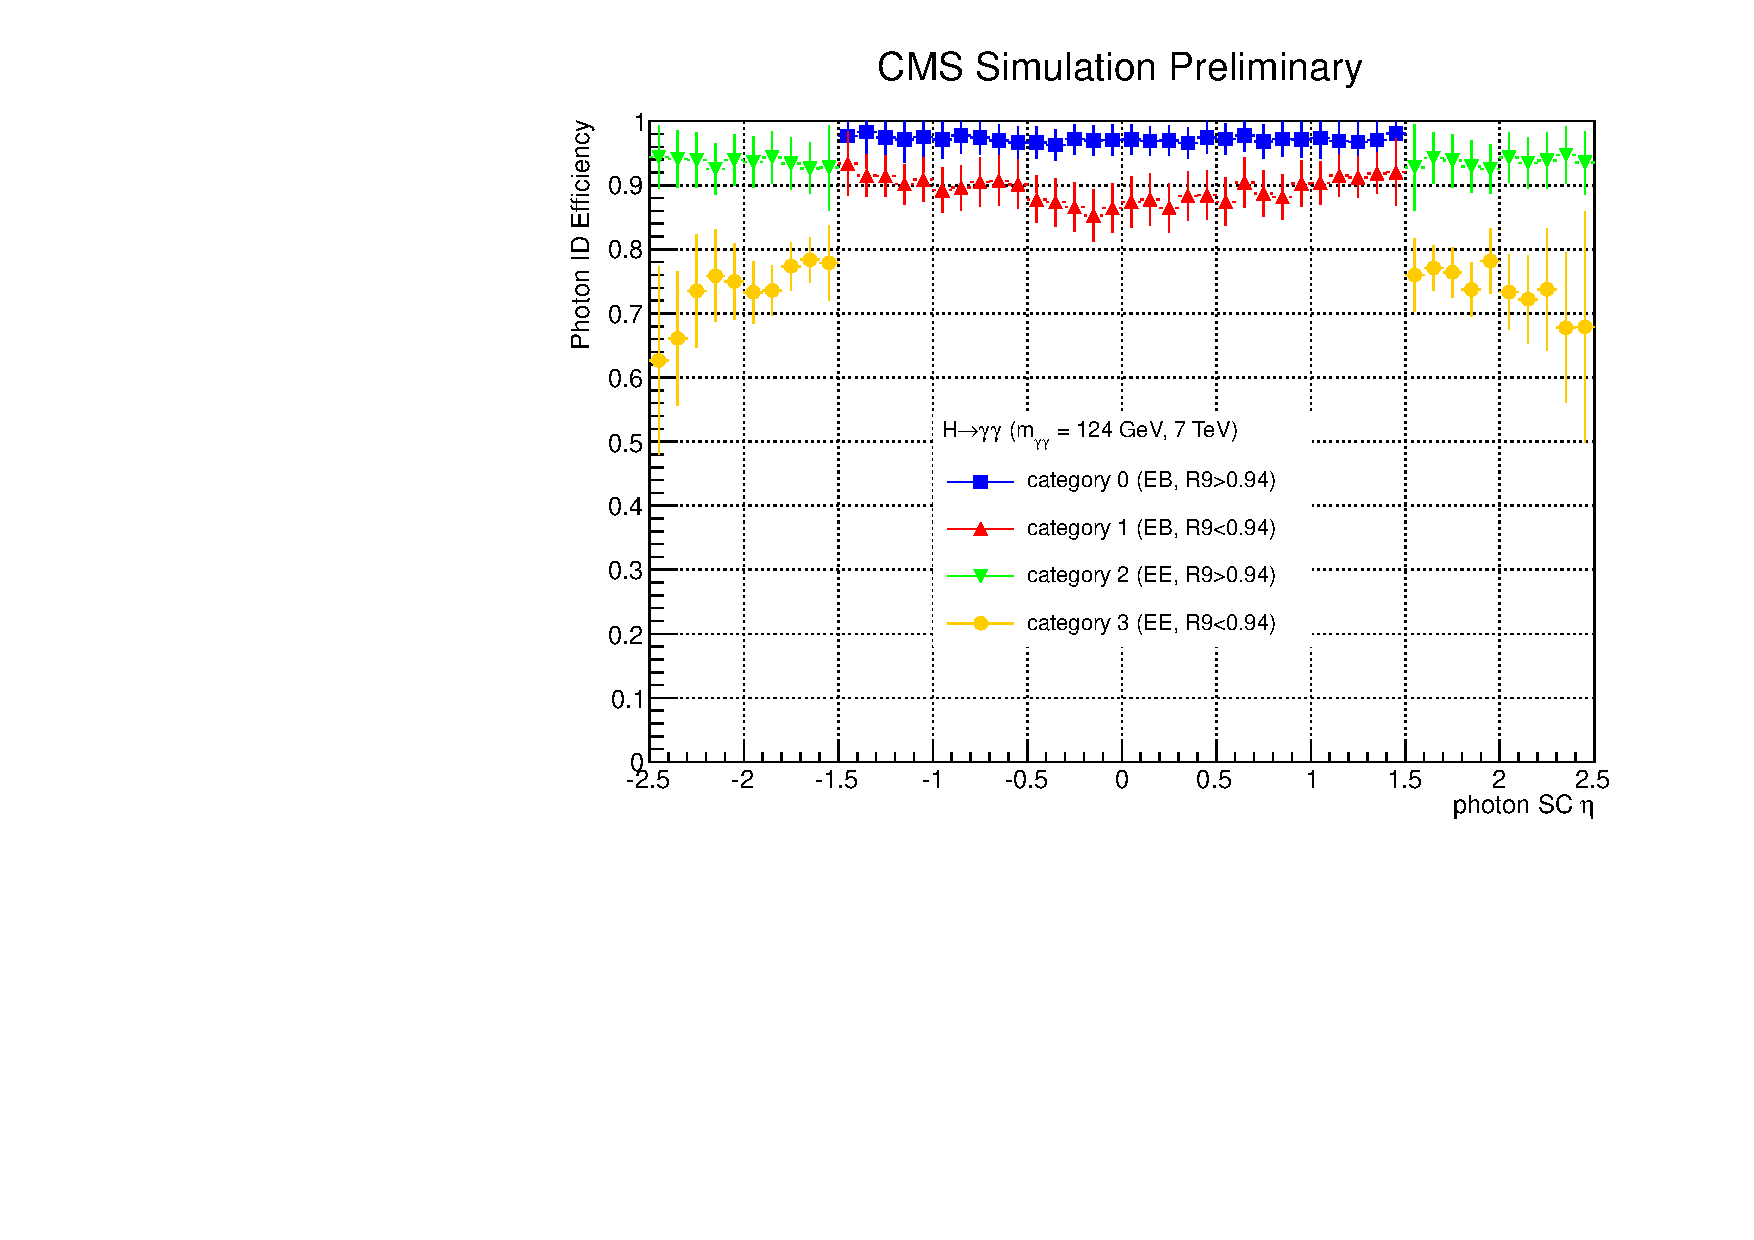
\includegraphics[width=0.48\textwidth]{ch4_selec_and_cats/plots/eff_7TeV_eta.pdf}
  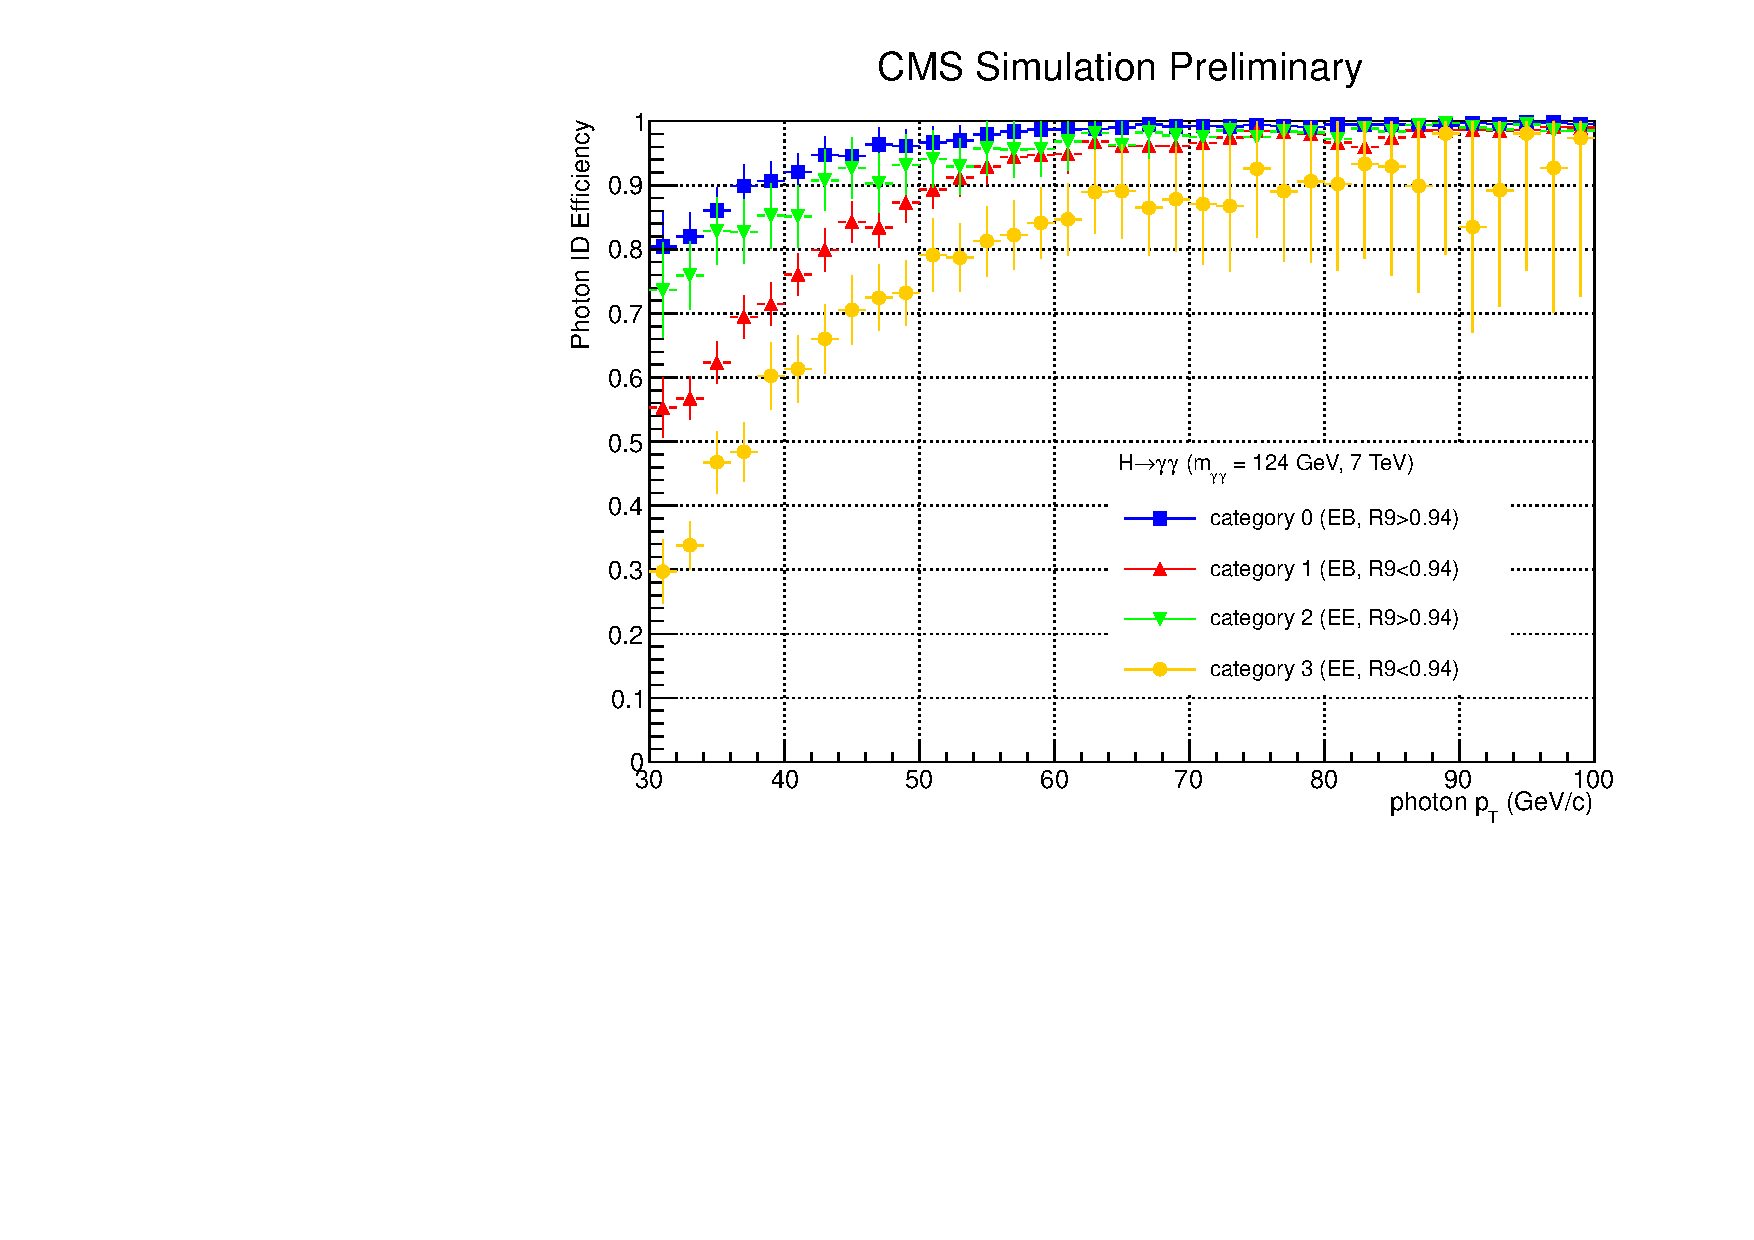
\includegraphics[width=0.48\textwidth]{ch4_selec_and_cats/plots/eff_7TeV_pt.pdf}
  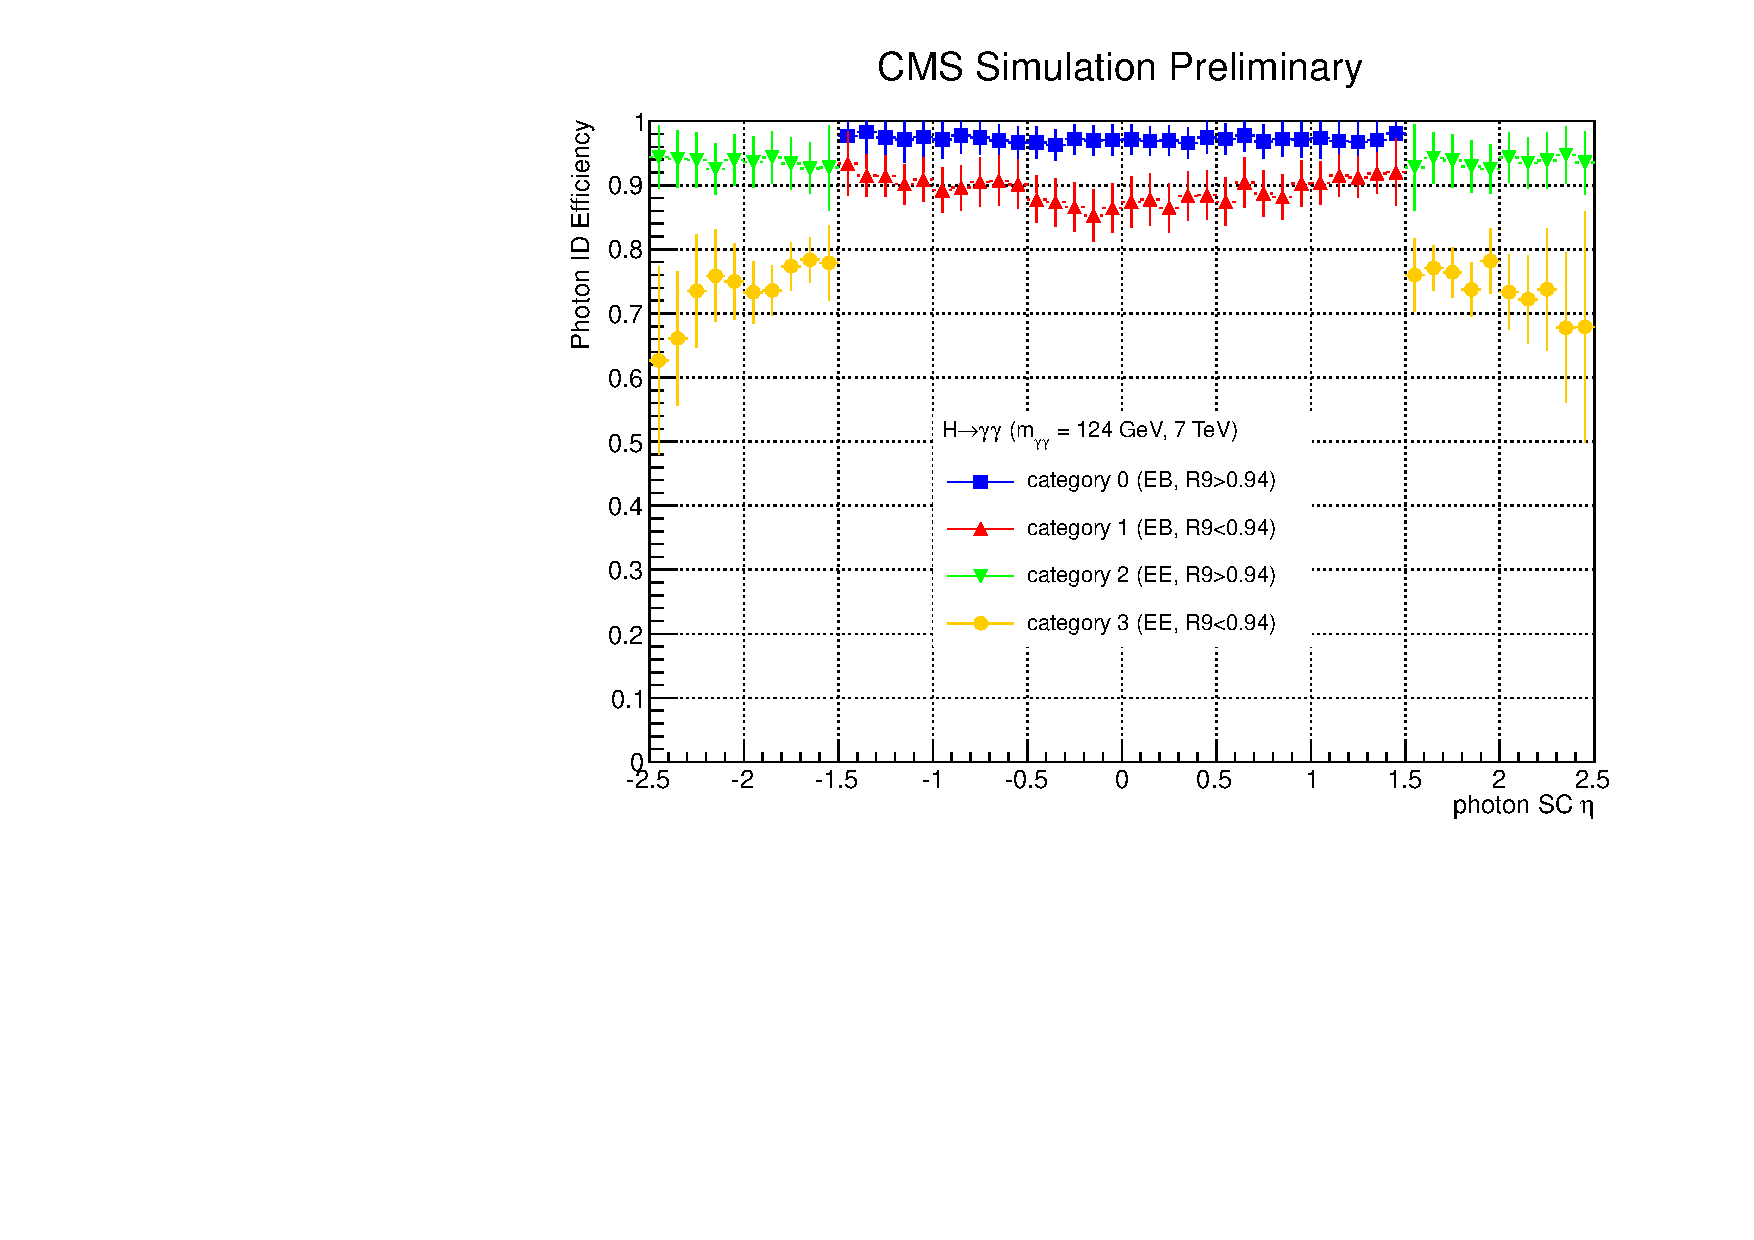
\includegraphics[width=0.48\textwidth]{ch4_selec_and_cats/plots/eff_7TeV_eta.pdf}
  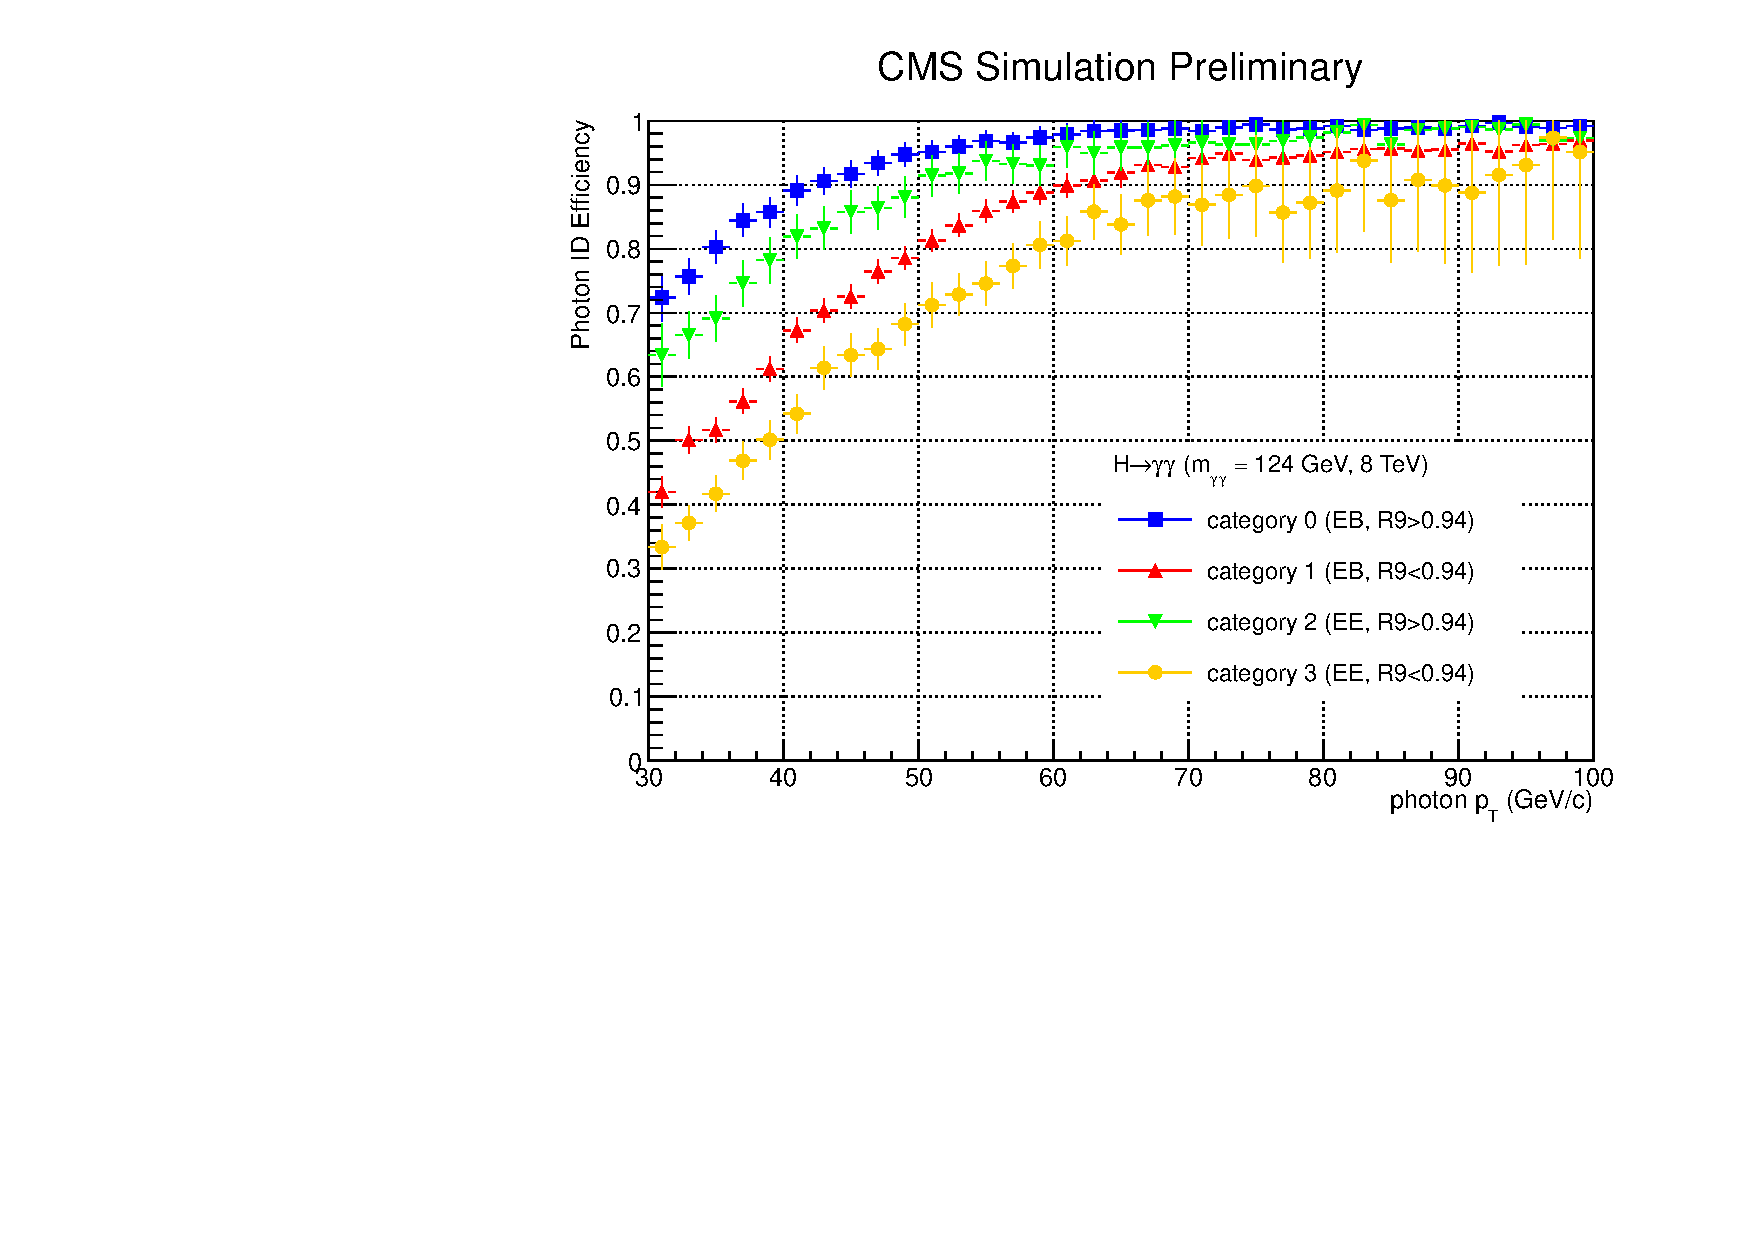
\includegraphics[width=0.48\textwidth]{ch4_selec_and_cats/plots/eff_8TeV_pt.pdf}
  \caption{Cut based photon ID efficiency as measured in \Zee tag and probe. MORE DESCRIPTION}
  \label{fig:cic_efficiency}
\end{figure}

\subsection{Photon ID MVA}
\label{sec:pho_id_mva}

For the multivariate approach a \BDT is trained to discriminate between prompt photons and jets. The desire is to factorise the photon selection, which is required to distinguish prompt photons from neutral mesons faking photons, and the event selection, which is required to consider kinematics, resolution etc.~to distinguish \Hgg from the $pp\rightarrow\gamma\gamma$ background. The input variables used are designed specifically to distinguish between prompt photons and neutral mesons faking photons to factorise out any event or photon kinematics which make the identification Higgs specific. Consequently, the training samples used are \gjet samples where the identification \BDT signal is the prompt $\gamma$ and the background is the fake jet. The \pT and supercluster \eta distribution of the prompt photon are reweighted to match the background non-prompt photons in order to further negate any photon kinematics which the \BDT could exploit. The photon ID \BDT is trained separately for the 7 and 8 \TeV and seperately for barrel and endcap as these regions of phase space are so different which results in four separate trainings in total.

The input variables aim to exploit differences in the shower shape and isolation between prompt and non-prompt photons and the correlation between these variables and the supercluster position and energy. They are,

\textbf{Shower shape variables}
\begin{itemize}
  \item $\sigma_{i\eta i\eta}$ - Explained above in Sec.~\ref{sec:photon_presel}
  \item $\sigma^{2}_{i\eta i\phi}$ - The diagonal spread (in \eta,\phi) of the shower.
  \item $E_{2\times2}/E_{5\times5}$ - Ratio of energy in the most energetic 2$\times$2 cluster which contains the seed to the energy in the 5$\times$5 cluster.
  \item $R_{9}$ - Explained above in Sec.~\ref{sec:ecal}.
  \item $\sigma_{\eta}$ - The energy weighted standard deviation of single crystal eta within the supercluster.
  \item $\sigma_{\phi}$ - The energy weighted standard deviation of single crystal phi within the supercluster.
  \item $\sigma_{RR}$ (for endcap only) - The standard deviation of the shower spread in the $x$, $y$ planes of the preshower.
\end{itemize}

\textbf{Isolation variables}
\begin{itemize}
  \item PF Photon ISO - Particle flow photon isolation sum
  \item PF Charged Hadron ISO (selected vertex) - Particle flow charged hadron isolation sum for candidate originating from selected vertex.
  \item PF Charged Hadron ISO (worst vertex - Particle flow charged hadron isolation sum for candidate originating from the vertex with the largest isoltion sum.
\end{itemize}

\textbf{Correlation variables}
\begin{itemize}
  \item $\rho$ - The median energy density in the event.
  \item $\eta$ - The \eta position of the photon supercluster.
  \item $E_{raw}$ - The raw energy of the photon supercluster.
\end{itemize}

The testing sample used to verify the output of the photon identification \BDT is a \MC \Hgg sample (\mH=124\GeV). The photon identification \BDT output (which is shown for the four different trainings in Figure~\ref{fig:photon_id_bdt}) provides a measure of an individual photons' ``quality" and is used as an input to the event level \BDT (described in the next section). Even so a considerable amount of background is cut out by defining a loose cut (the \BDT output must be $>-0.2$) on the photon ID \BDT output value which is more than 95\% signal efficient.

The photon ID \BDT response for each photon is used as a direct input to the event level \MVA. Given that imperfect modeling of the detector response can result in a small change in the photon ID response which has a direct impact on the event level \MVA response, which is used to classify events, a systematic on the photon quality is applied and propagated through to the event level \MVA. Validation of the photon ID \BDT response in the \Zee decay is shown in Figure~\ref{fig:photon_id_zee} with the size of the systematic shown. Validation is done with the \Zee decay on all of the input variables, these distributions are shown in Appendix~\ref{app:photon_id} (\red{this may not be entirely necessary})


\begin{figure}
  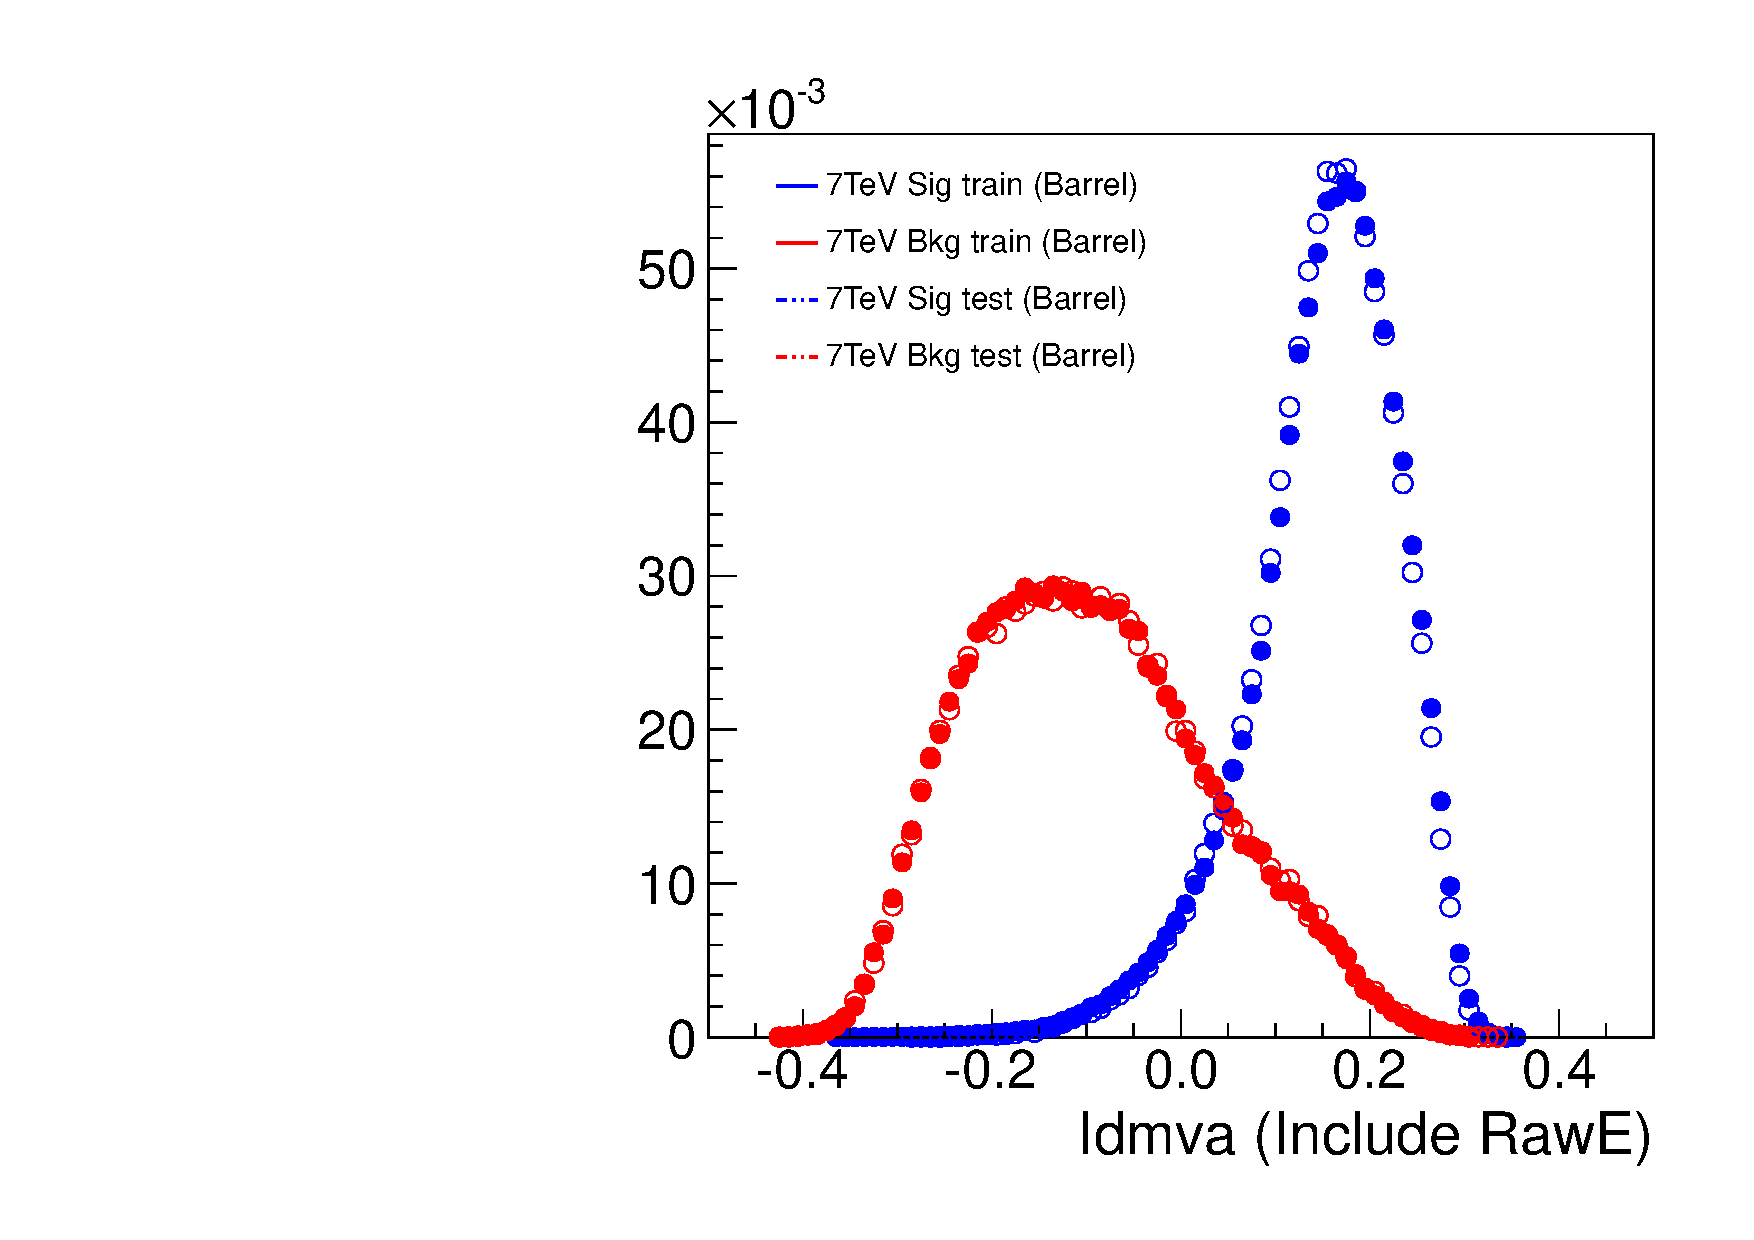
\includegraphics[width=0.48\textwidth]{ch4_selec_and_cats/plots/photonID_7TeV_barrel.pdf}
  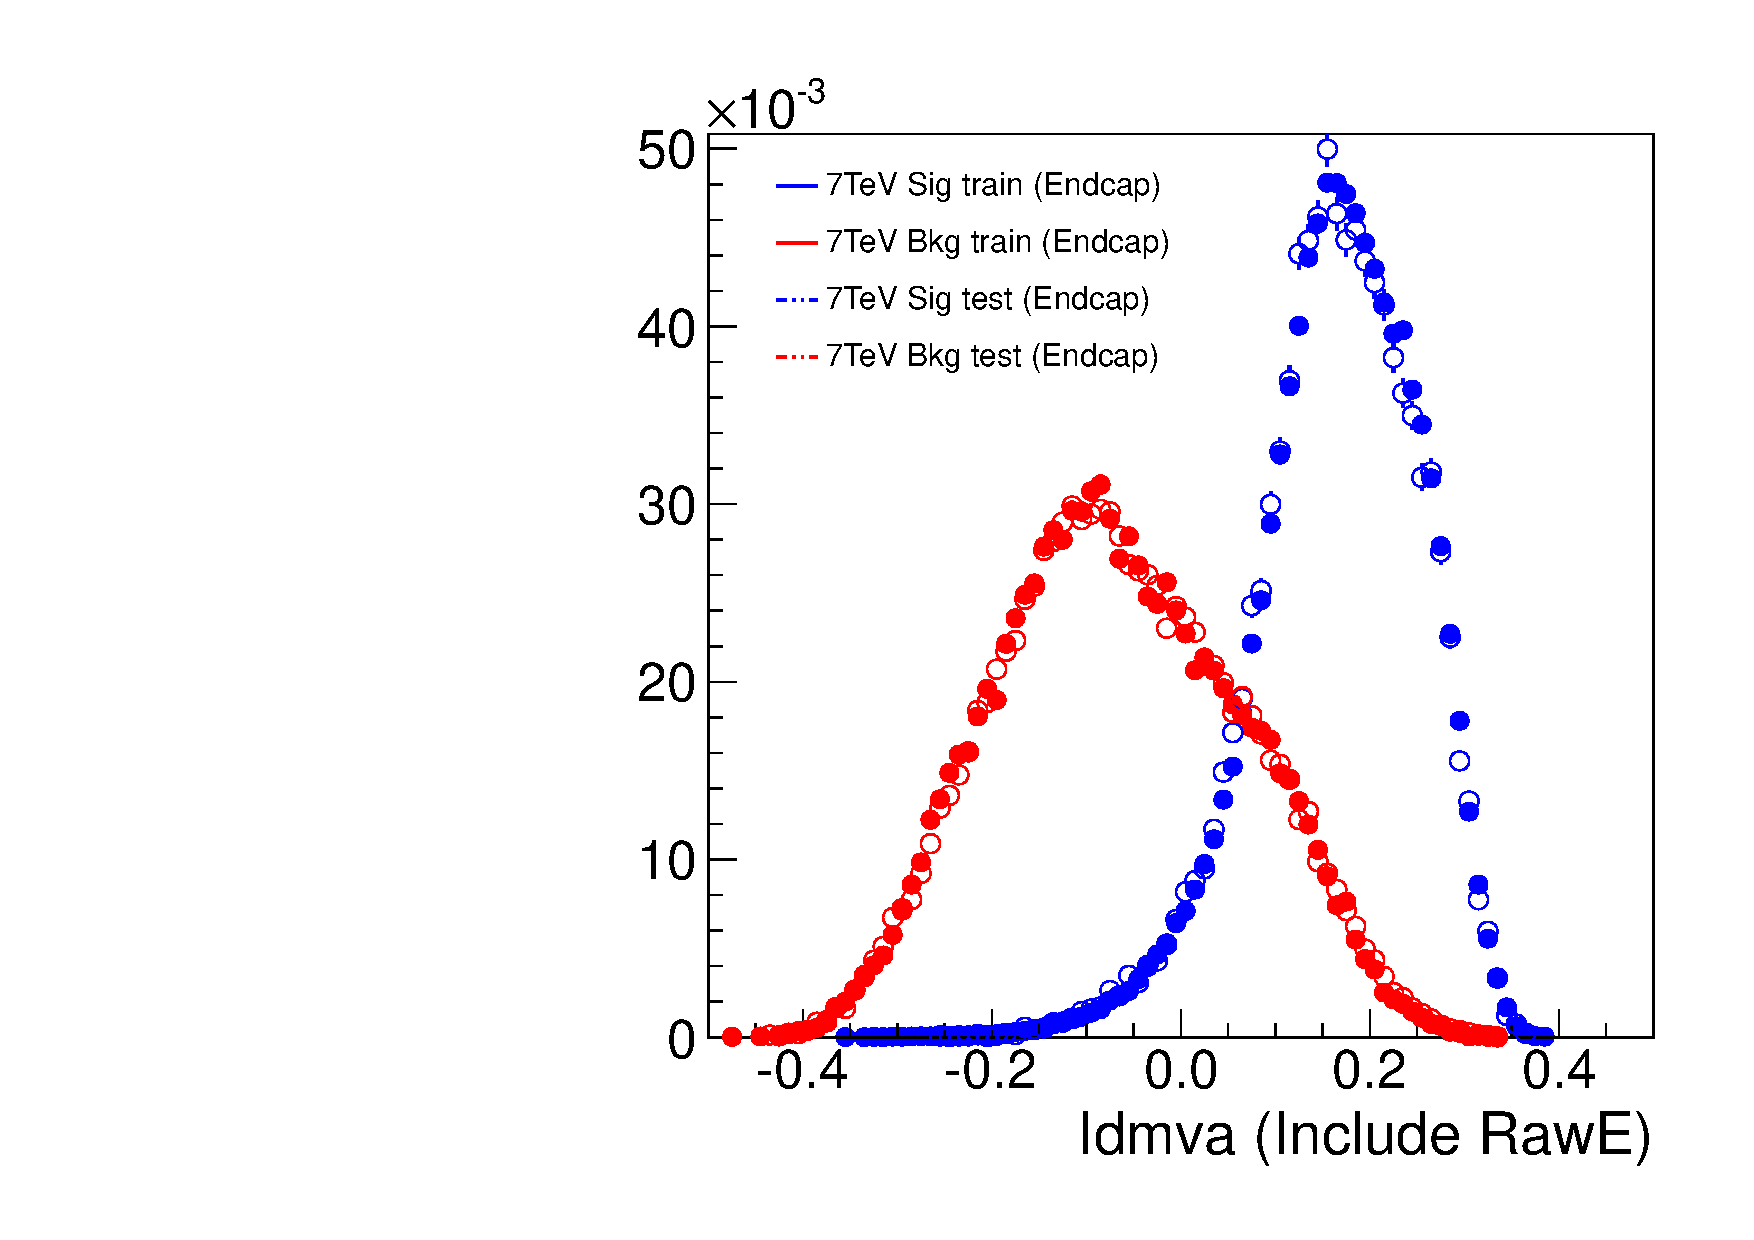
\includegraphics[width=0.48\textwidth]{ch4_selec_and_cats/plots/photonID_7TeV_endcap.pdf} \\
  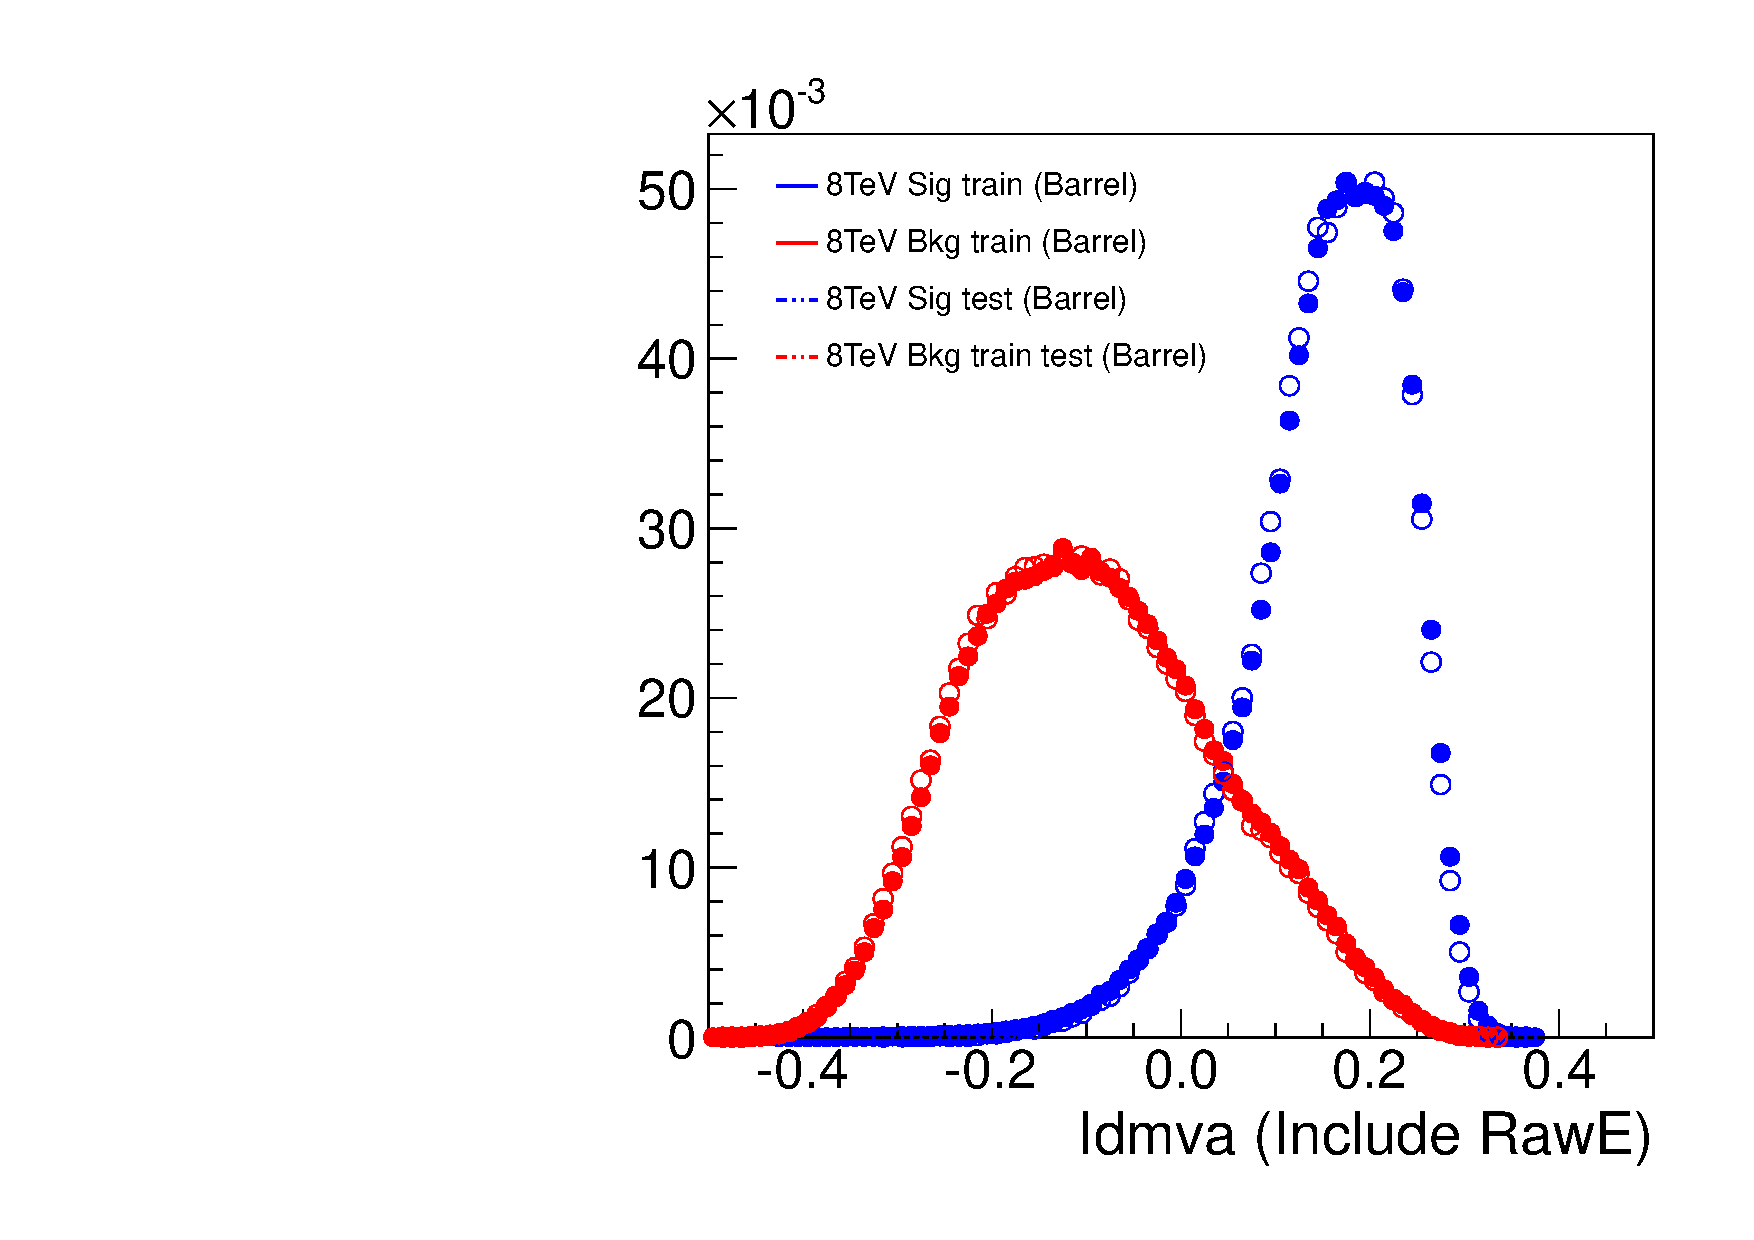
\includegraphics[width=0.48\textwidth]{ch4_selec_and_cats/plots/photonID_8TeV_barrel.pdf}
  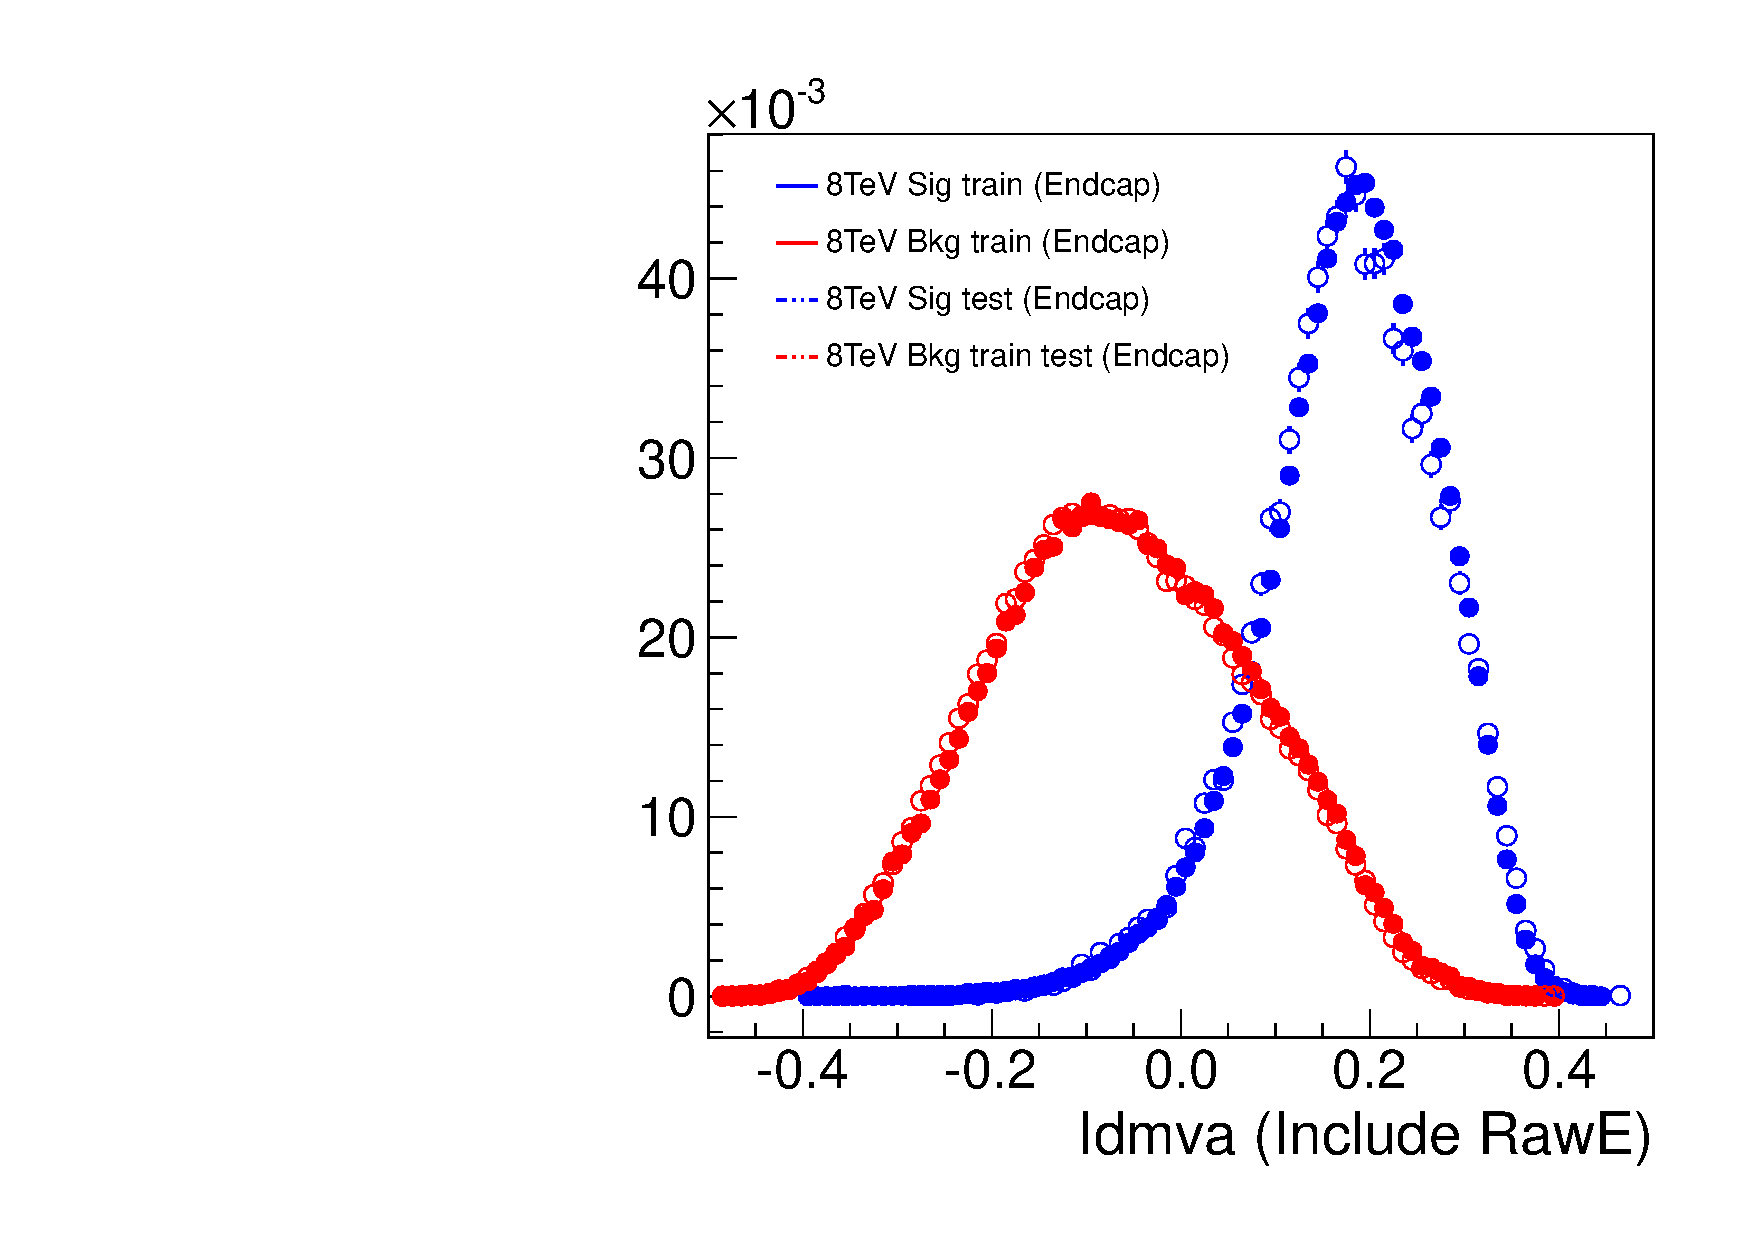
\includegraphics[width=0.48\textwidth]{ch4_selec_and_cats/plots/photonID_8TeV_endcap.pdf}
  \caption{The output distribution of the photon identification \BDT for 7\TeV barrel (top left), 7\TeV endcap (top right), 8\TeV barrel (bottom left) and 8\TeV endcap (bottom right). The solid points show the \gjet training sample distributions and the hollow points show the \Hgg test sample distributions for prompt signal photons in blue and fake background photons in red. A cut of $>-0.2$ is made on all photons.}
  \label{fig:photon_id_bdt}
\end{figure}

\begin{figure}
  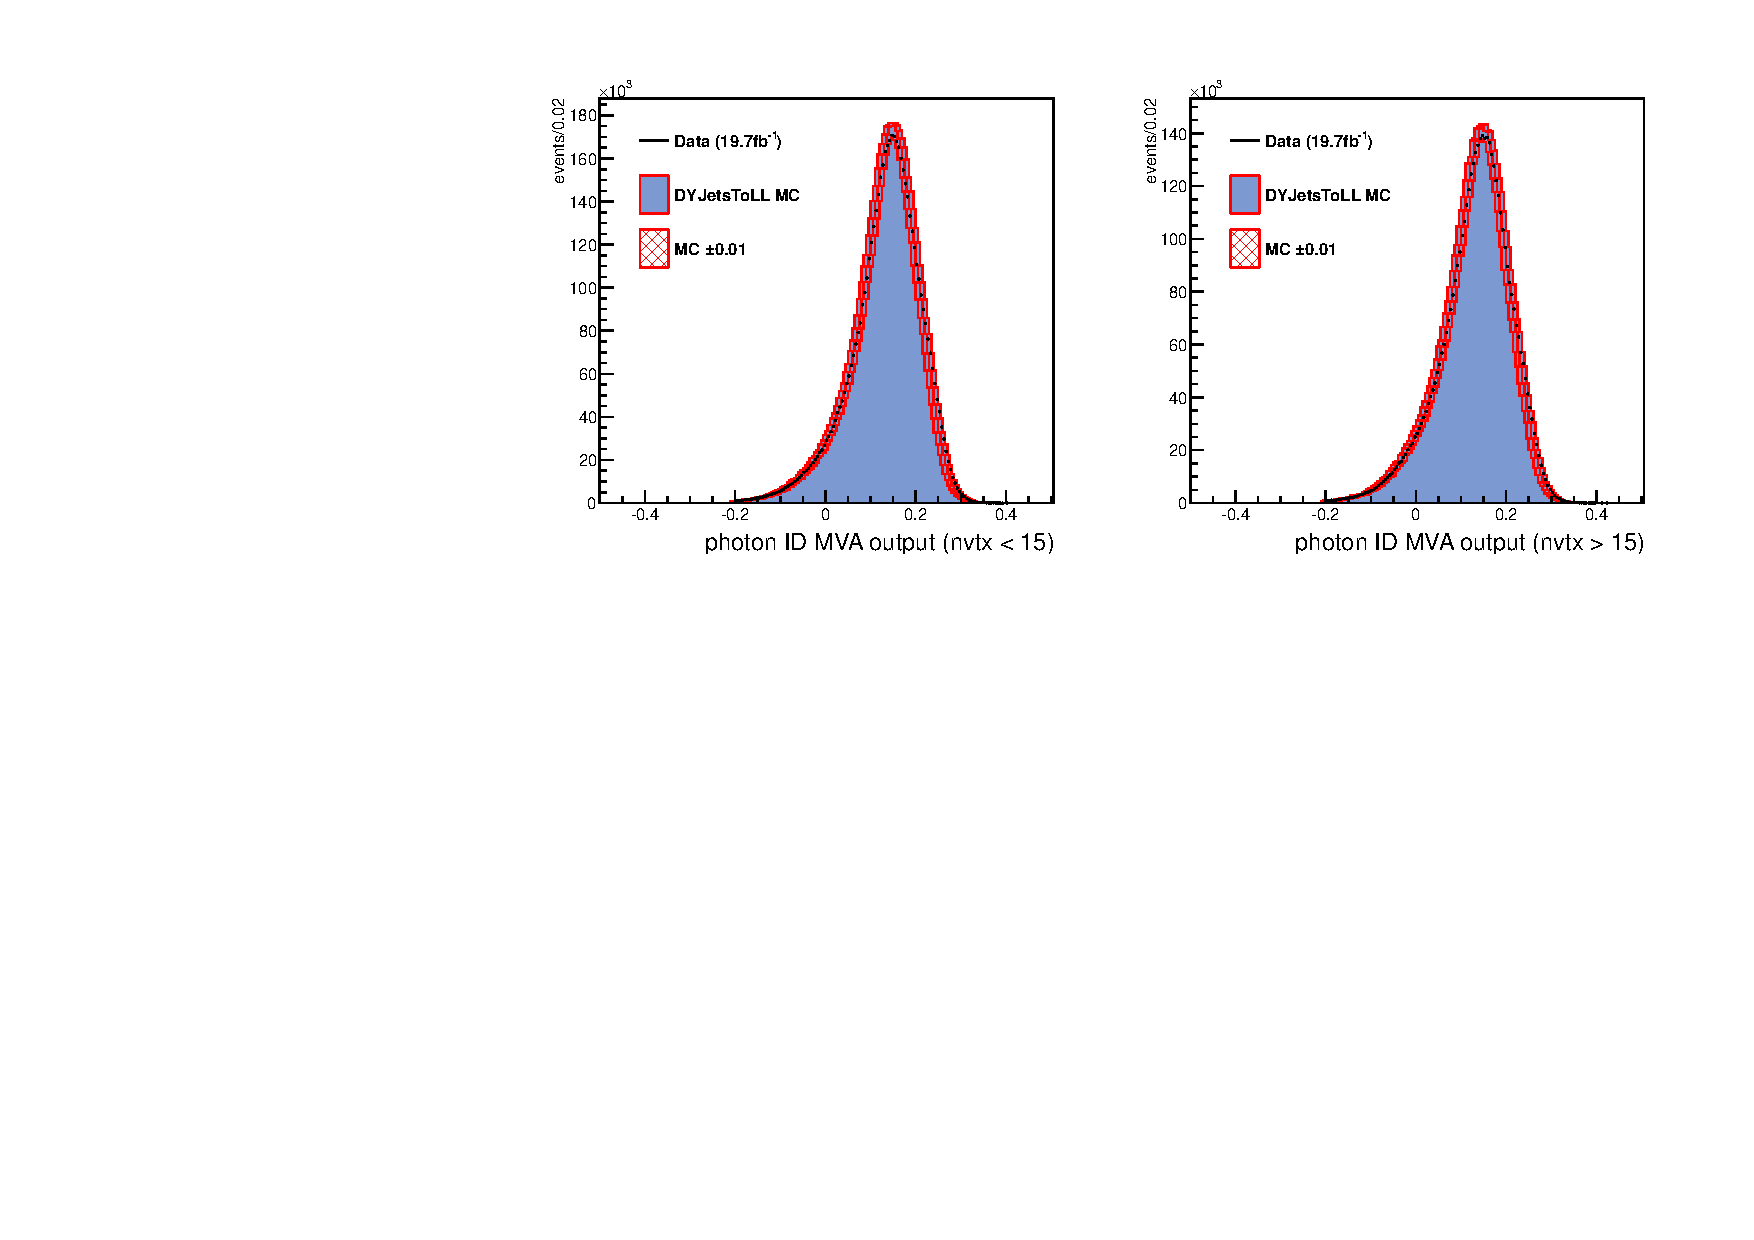
\includegraphics[width=0.48\textwidth]{ch4_selec_and_cats/plots/photonID_zee_8TeV.pdf}
  \caption{The output distribution of the photon identification \BDT for the 8~\TeV training as validated by the \Zee decay. The data is shown as the black points with the \MC as the blue histogram. The systematic uncertainty on the output as applied to the \MC is shown as the red band. \red{This is literally just a place holder for the plot that I want to show.}}
  \label{fig:photon_id_zee}
\end{figure}

\subsection{Diphoton event level MVA}
\label{sec:diphoton_bdt}

Whilst the CiC analysis selects events based on photon identification, the \MVA analysis approach is to first select photons using the photon identification \BDT described in the section above and then pass all the relevant event information through an event level \BDT. The event level classifier is constructed to give a high score to events which fulfill the following criteria:

\begin{enumerate}
  \item The event kinematics should be compatible with a Higgs decay,
  \item The event has good mass resolution,
  \item The event contains two ``high quality" photons (i.e.~they have a high score from the photon ID \BDT).
\end{enumerate}

It is highly important that the \BDT is completely independent of Higgs mass and that the input variables use have no, or at the least very little, dependence on the Higgs mass. This is essential to have a fair training. For example if the \BDT included the Higgs mass, or a variable highly correlated with it, it would preferentially select events with this mass therefore biasing the selection towards events which have a mass near the mass of the signal used to train with. The input variables used are,

\textbf{Event kinematics}
\begin{itemize}
  \item $p_{T}^{1(2)}/m_{\gamma\gamma}$ - The mass relative transverse momenta of each photon.
  \item $\eta^{1(2)}$ - The pseudorapidity of each photon.
  \item $\cos(\phi_{1}-\phi_{2})$ - The cosine of the angle between the two photons in the transverse plane. This variable reflects the \pT of the diphoton system (in other words the Higgs) without introducing a mass dependence.
\end{itemize}

\textbf{Mass resolution}
\begin{itemize}
  \item $\sigma_{m}^{right}/m_{\gamma\gamma}$ - The mass resolution of the event assuming the correct primary vertex has been selected. In this case the angular resolution is neglible so the variable is caluclated using just the two photon energy resolution values as,
    \begin{equation}
      \frac{\sigma_{m}^{right}}{m_{\gamma\gamma}} = \frac{1}{2}\Bigl(\frac{\sigma_{E_{1}}}{E_{1}} \oplus \frac{\sigma_{E_{2}}}{E_{2}}\Bigr).
    \end{equation}
  \item $\sigma_{m}^{wrong}/m_{\gamma\gamma}$ - The mass resolution of the event assuming the wrong vertex is selected. The vertex position in $z$ is distributed as a Gaussian with a width equivalent to $\sqrt{2}\sigma_{z}^{beamspot}$ and so the angular resolution $\sigma_{m}^{vtx}$ can be analytically calculated given the \ECAL impact positions of the two photons. Consequently the wrong vertex variable is calculated as,
    \begin{equation}
      \frac{\sigma_{m}^{wrong}}{m_{\gamma\gamma}} = \frac{\sigma_{m}^{right}}{m_{\gamma\gamma}} \oplus \frac{\sigma_{m}^{vtx}}{m_{\gamma\gamma}}.
    \end{equation}
  \item $p_{vtx}$ - The probability that the selected primary vertex is correct. In order to tie together the mass resolution information given the right vertex hypothesis and the wrong vertex hypothesis, the probability that the vertex is correct is used in addition.
  \item It is also important to specify in the training that the signal to background ratio is inversely proportional to the mass resolution. Accordingly the signal events in the training are weighted by a factor,
    \begin{equation}
      w = \frac{p_{vtx}}{\sigma_{m}^{right}/m_{\gamma\gamma}} + \frac{1-p_{vtx}}{\sigma_{m}^{wrong}/m_{\gamma\gamma}}.
    \end{equation}
\end{itemize}

\textbf{Photon quality}
\begin{itemize}
  \item $phoID^{1(2)}$ - The photon ID \BDT output value of each photon.
\end{itemize}

The training is performed separately for 7 and 8~\TeV and the samples used for the signal are all of the \SM \Hgg \MC samples ($ggH$, $qqH$, $WZH$, $ttH$) appropriately weighted by cross section and the samples used for the background are the cross section weighted mixture of \SM backgrounds which include contributions from $pp\rightarrow\gamma\gamma$ (prompt-prompt), $pp\rightarrow\gamma\mbox{jet}$ (prompt-fake) and $pp\rightarrow\mbox{jet~jet}$ (fake-fake) as described in Sec.~\ref{sec:mc}. The training is performed on only half of the event samples (selected by even event number) so that the BDT response can be tested on the other half (selected by odd event number).

A cut is placed on the \BDT response in order to remove almost all the events which contain two fake photons. The remaining events which pass this cut are categorised in coarse bins based the on the \BDT response as explained in the following section. The \BDT response in data, background and signal is shown in Figure~\ref{fig:dipho_bdt}. The cut values are $>0.19$ for the 7~\TeV training and $>-0.78$ for the 8~\TeV training. It can be seen from this figure that the cut on the event level \BDT removes nearly all of the fake-fake contribution to the background whilst the remaining fractions consist of about 70\% prompt-prompt and 30\% prompt-fake.

\begin{figure}
  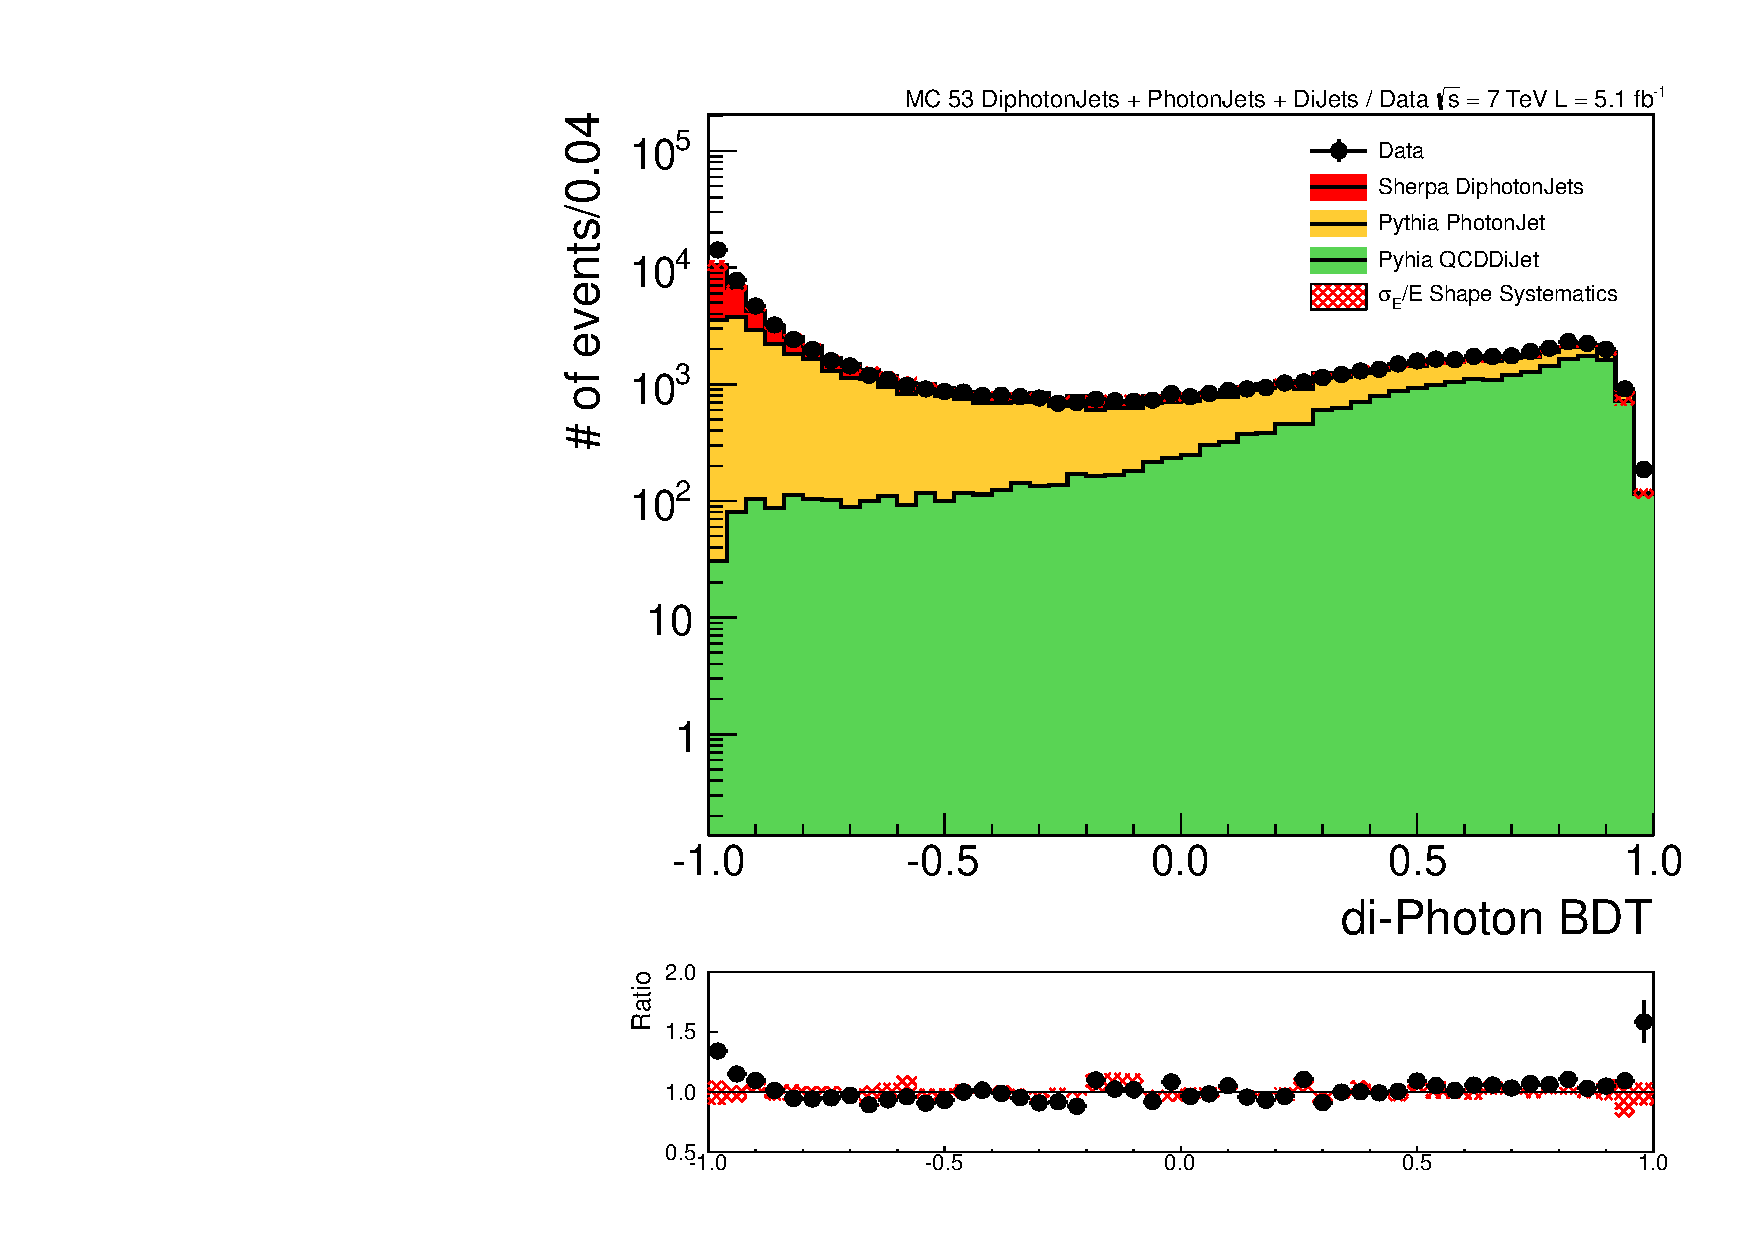
\includegraphics[width=0.48\textwidth]{ch4_selec_and_cats/plots/diphoBDT_7TeV_bkg.pdf}
  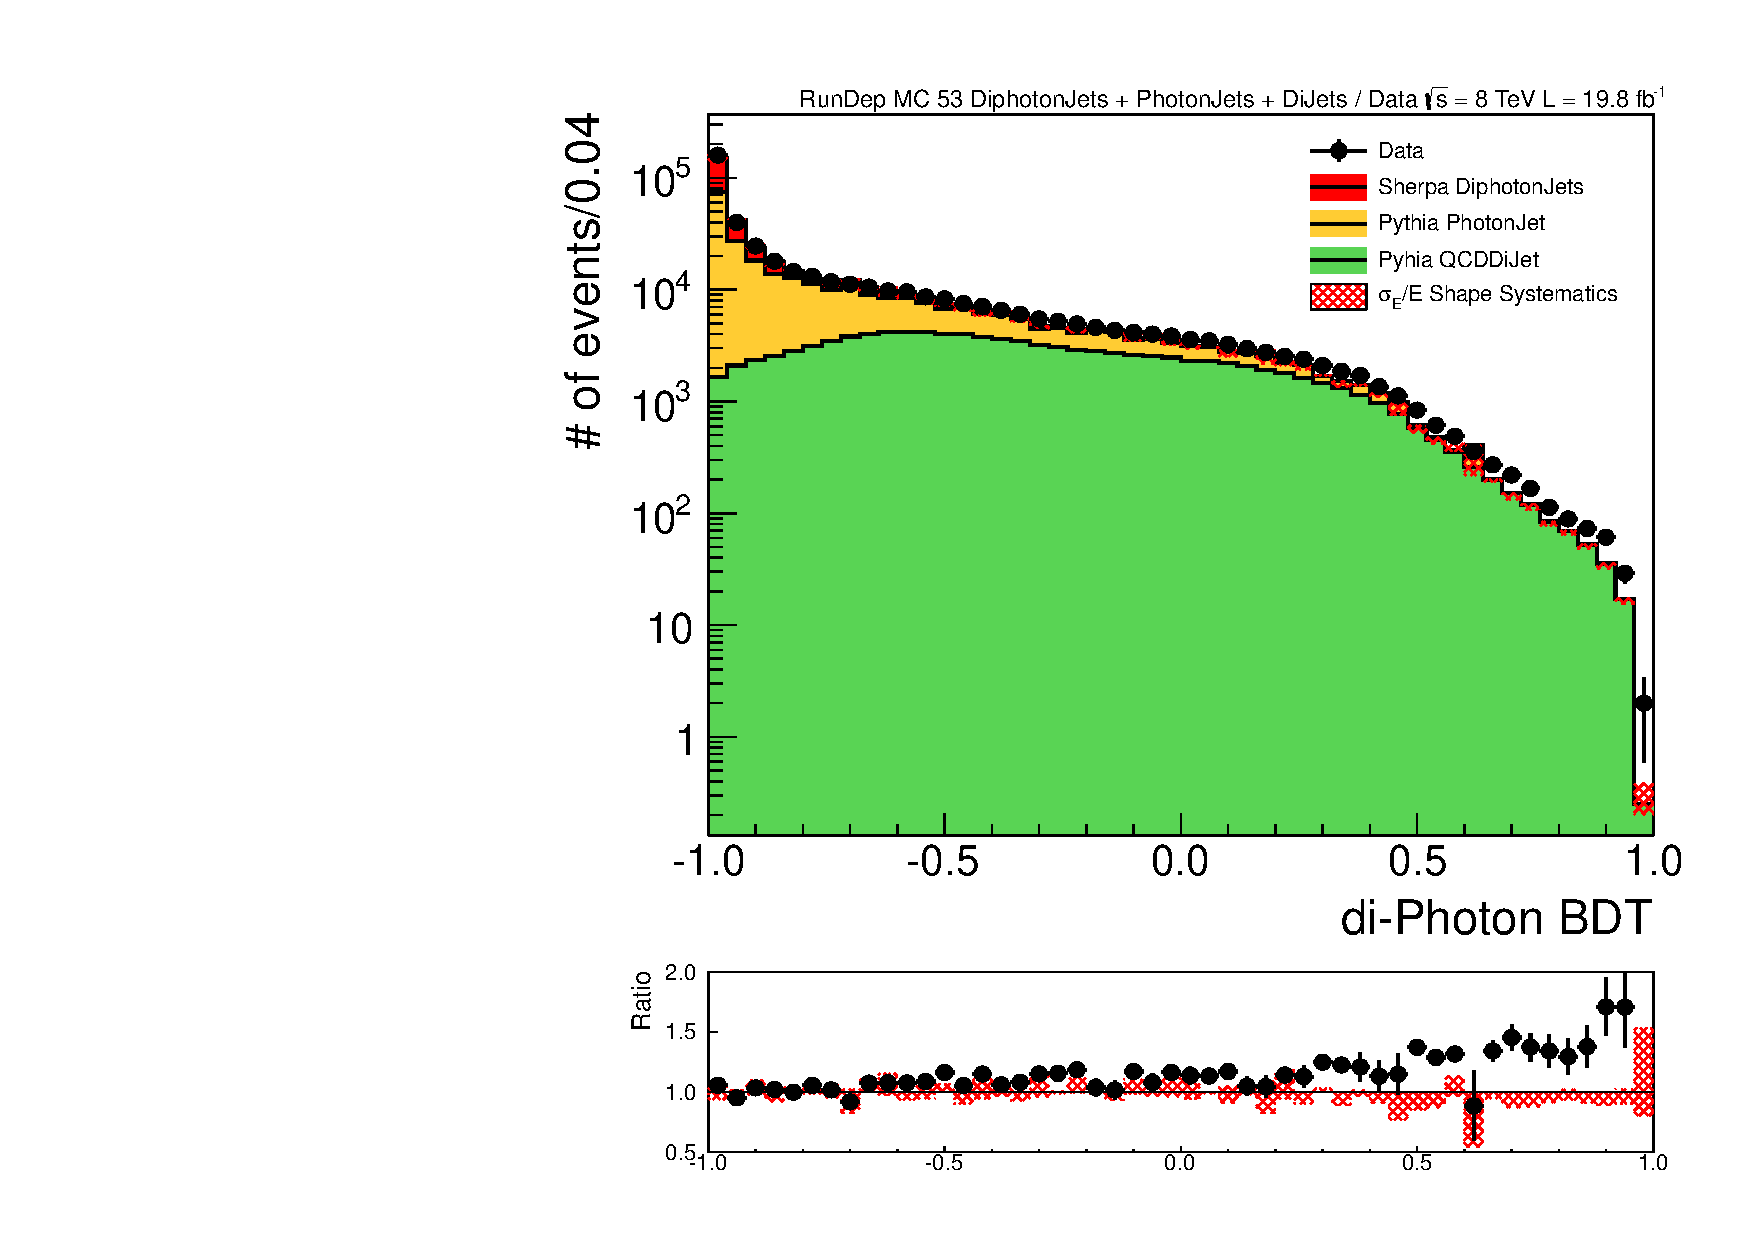
\includegraphics[width=0.48\textwidth]{ch4_selec_and_cats/plots/diphoBDT_8TeV_bkg.pdf} \\
  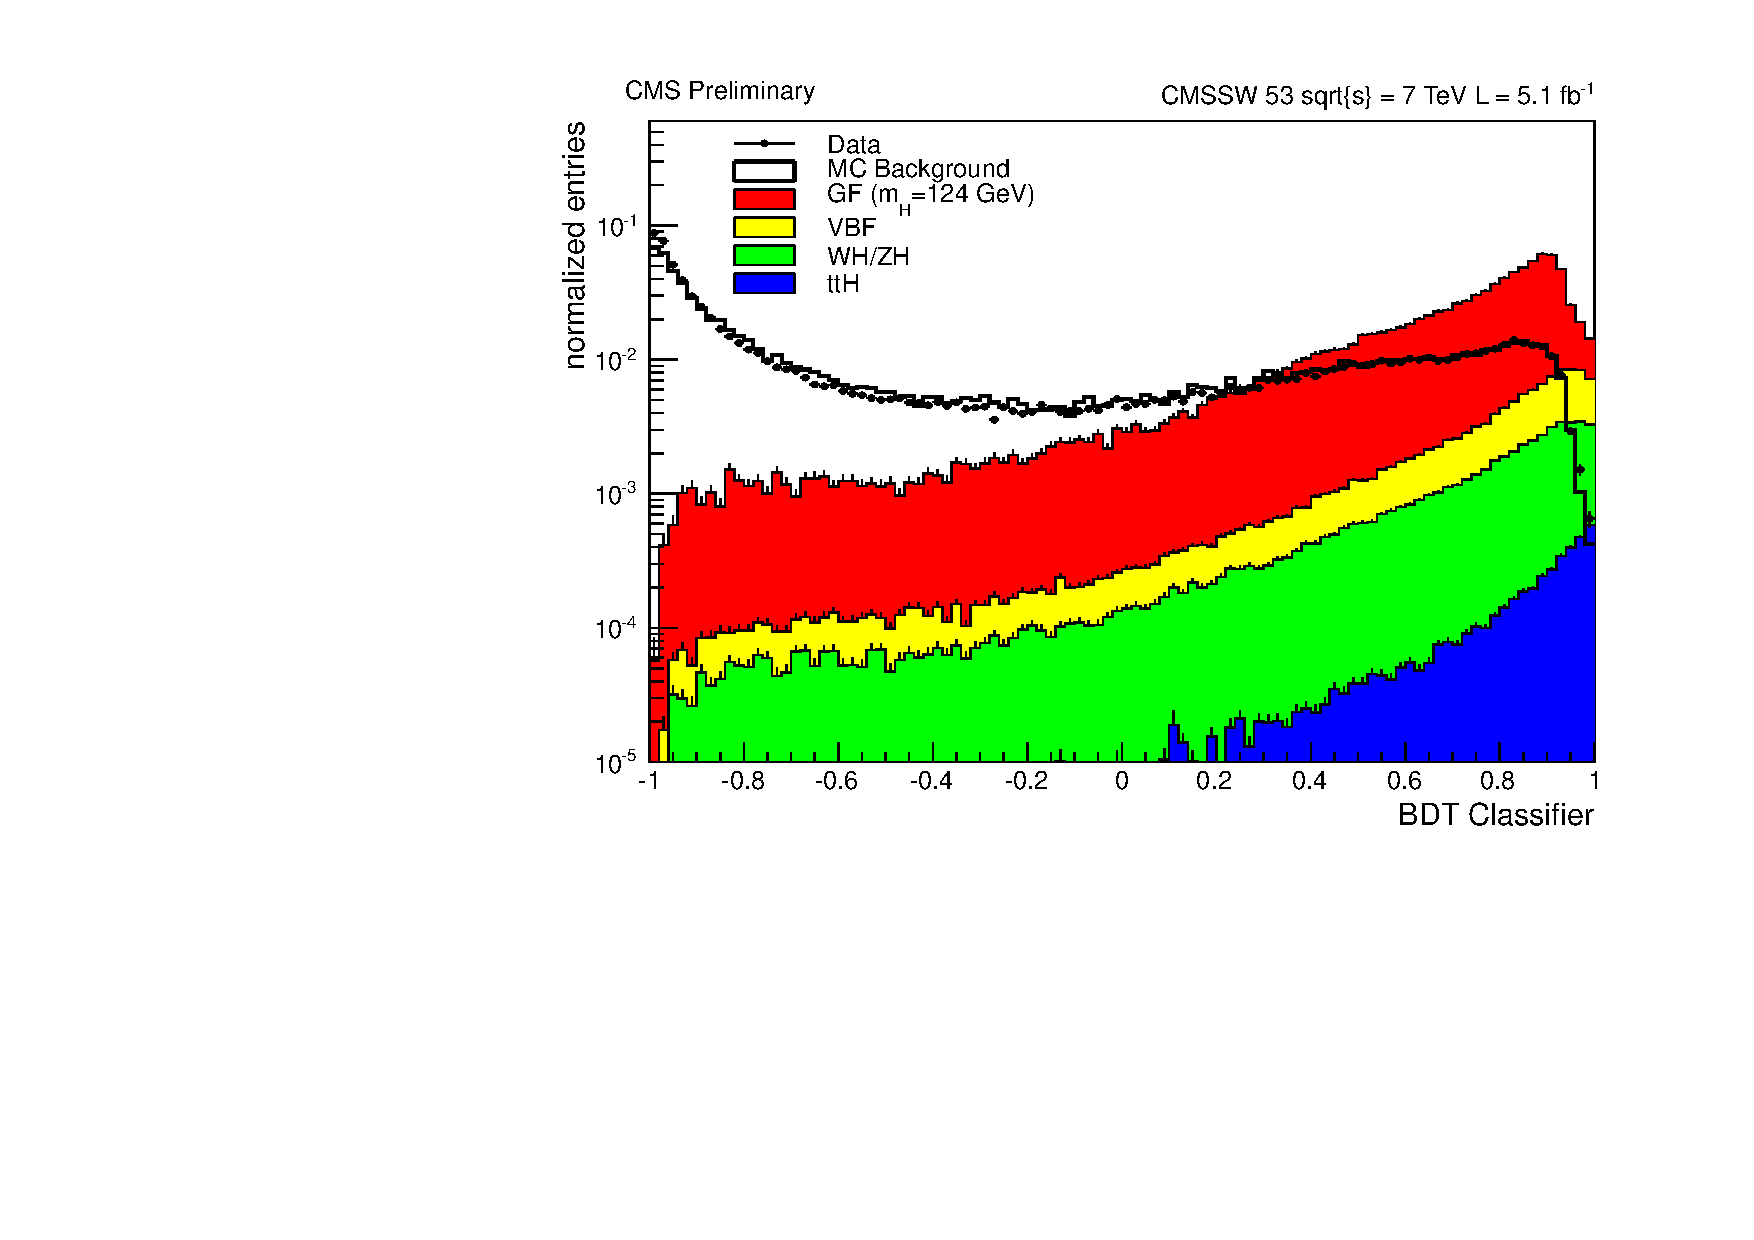
\includegraphics[width=0.48\textwidth]{ch4_selec_and_cats/plots/diphoBDT_7TeV_sig.pdf} 
  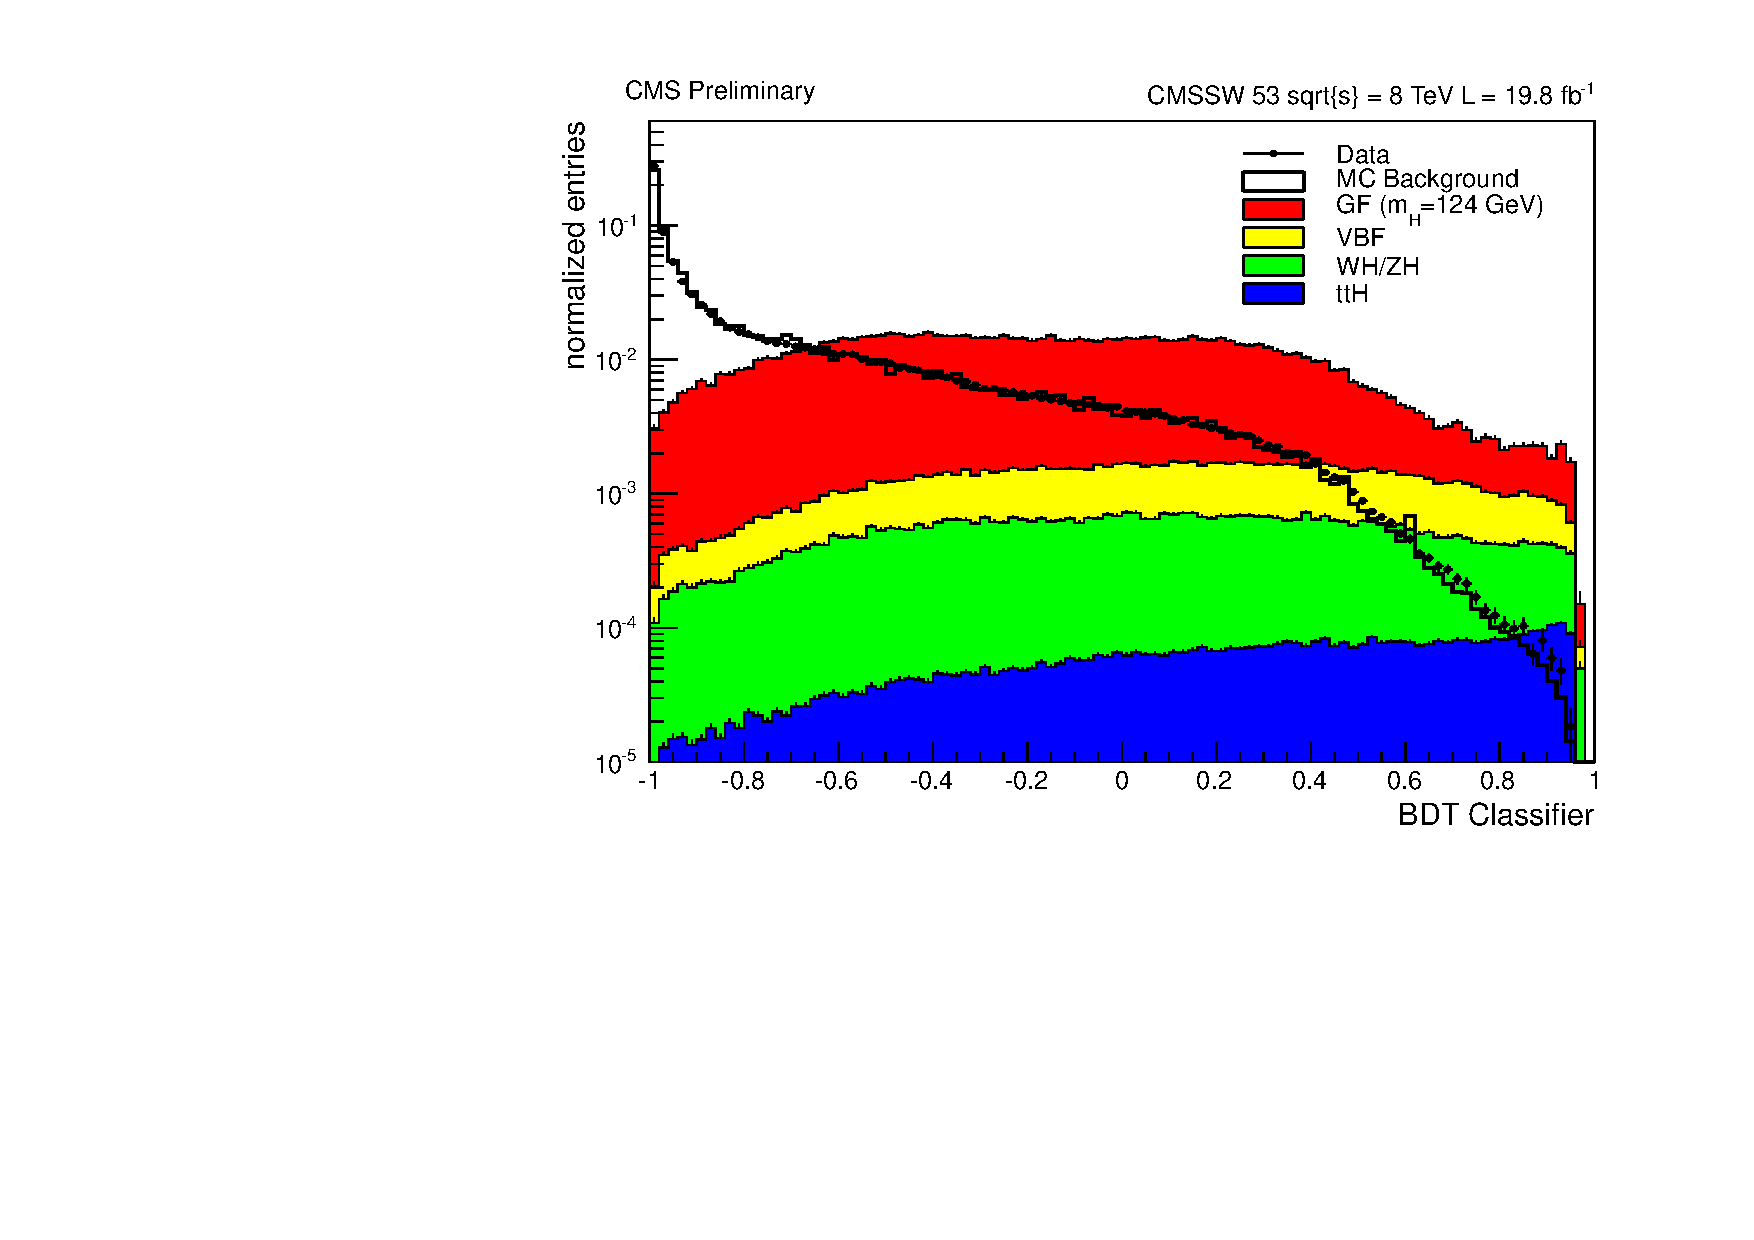
\includegraphics[width=0.48\textwidth]{ch4_selec_and_cats/plots/diphoBDT_8TeV_sig.pdf}
  \caption{The diphoton BDT response for the 7~\TeV training (left column) and 8~\TeV training (right column). The data and background distributions are shown in the plots on the top row for data in the range $100 < m_{\gamma\gamma} < 120$~\GeV and $130 < m_{\gamma\gamma} < 180$~\GeV (black points) and for the prompt-prompt background (green), prompt-fake background (yellow) and fake-fake background (red). The signal distributions are shown in the plots on the bottom row for gluon fusion (red), vector boson fusion (yellow), associated $W$, $Z$ production (green) and associated $t\bar{t}$ production (blue) alongside the data in the range $100 < m_{\gamma\gamma} < 120$~\GeV and $130 < m_{\gamma\gamma} < 180$~\GeV (black points) and the total background (hollow histogram). \red{PLOTS NEED UPDATING}}
  \label{fig:dipho_bdt}
\end{figure}

Whilst the background in this analysis is obtained in a completely data driven way the signal model is obtained from \MC. Consequently any uncertainties which effect the shape of the output distribution of this \BDT in the signal result in event migrations between the final analysis categories. The input variables whose uncertainties have the largest effect on the \BDT response in signal are the photon ID quality and the photon energy resolution estimate. This is because these variables have both i) relatively large uncertainties because of imperfect detector response modelling in the simulation and ii) are highly discrimative and hence can have a relatively large impact on the \BDT response. As these variables both vary monotonically with the \BDT response the sytematic uncertainty on them is propagated through the analysis as an event migration. The size of this effect is shown in the \BDT response validation plot with the \Zee decay in Figure~\ref{fig:diphotonBDT_zee}. Validation plots using the \Zee channel for each of the event level \BDT input variables is shown in Appendix~\ref{app:diphoton_bdt} (\red{may not be necessary}).

\begin{figure}
  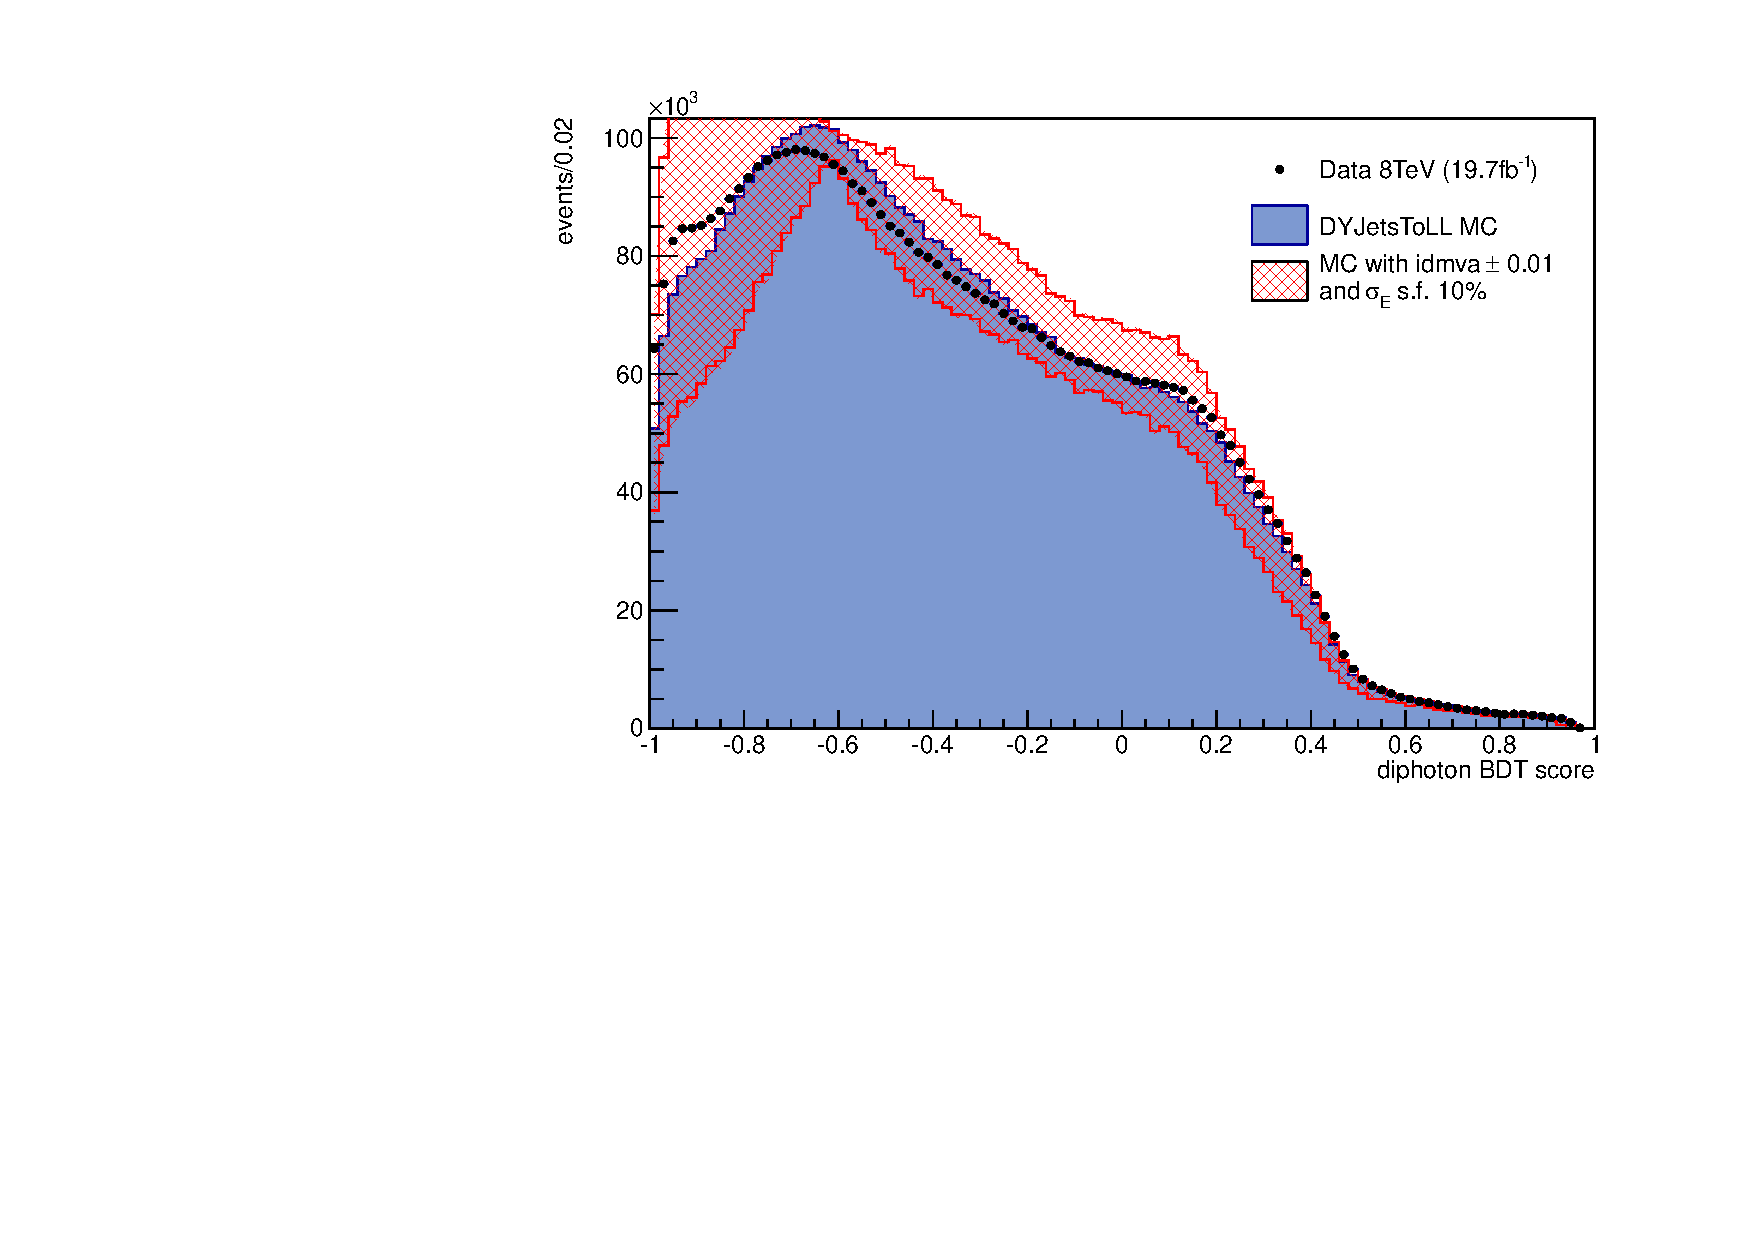
\includegraphics[width=0.6\textwidth]{ch4_selec_and_cats/plots/diphoBDT_8TeV_zee.pdf}
  \caption{The diphoton BDT response for the 8~\TeV training in the \Zee decay. The data is shown as the black points and the \MC as the blue histogram. The systematic applied to account for variation in the BDT response from mismodelling in the photon quality response and the photon energy resolution estimate are shown as the red band. \red{This is just a placeholder for the plot I want to show}}
  \label{fig:diphotonBDT_zee}
\end{figure}

% ---- SECTION ----
\section{Event categorisation}
\label{sec:categorisation}

  \subsection{Exclusive mode tagging}
  \label{sec:exclusive_tags}

  \subsection{Inclusive mode categorisation in the mass factorised analysis}
  \label{sec:inclusive_cats_massfac}

  \subsection{Inclusive mode categorisation in the sideband analysis}
  \label{sec:invlusive_cats_sideband}

